% Chapter 1
\setchapterimage{jet}
\setchapterpreamble[u]{\margintoc}
\chapter{Fusion: general introduction}\label{Chapter1}
% For referencing the chapter elsewhere, use \ref{Chapter1} 


\section{Thermonuclear fusion}

The fundamental principle of nuclear fusion is to fuse two light nuclei into a heavier nucleus.
The mass difference between the products and the reactants is released in the form of energy (see \refeq{emc2}).
\begin{equation}
    E = \Delta m c^2
    \labeq{emc2}
\end{equation}
where $\Delta m$ is the mass difference, $c$ is the speed of light in vacuum.
This process is the opposite process of nuclear fission, powering the current nuclear plants.

When looking at the different binding energies per nucleon of the elements (see \reffig{binding energy per nucleon}), it becomes clear that light elements release energy from fusion and heavy elements release energy from fission.

\begin{figure} [h]
    \centering
    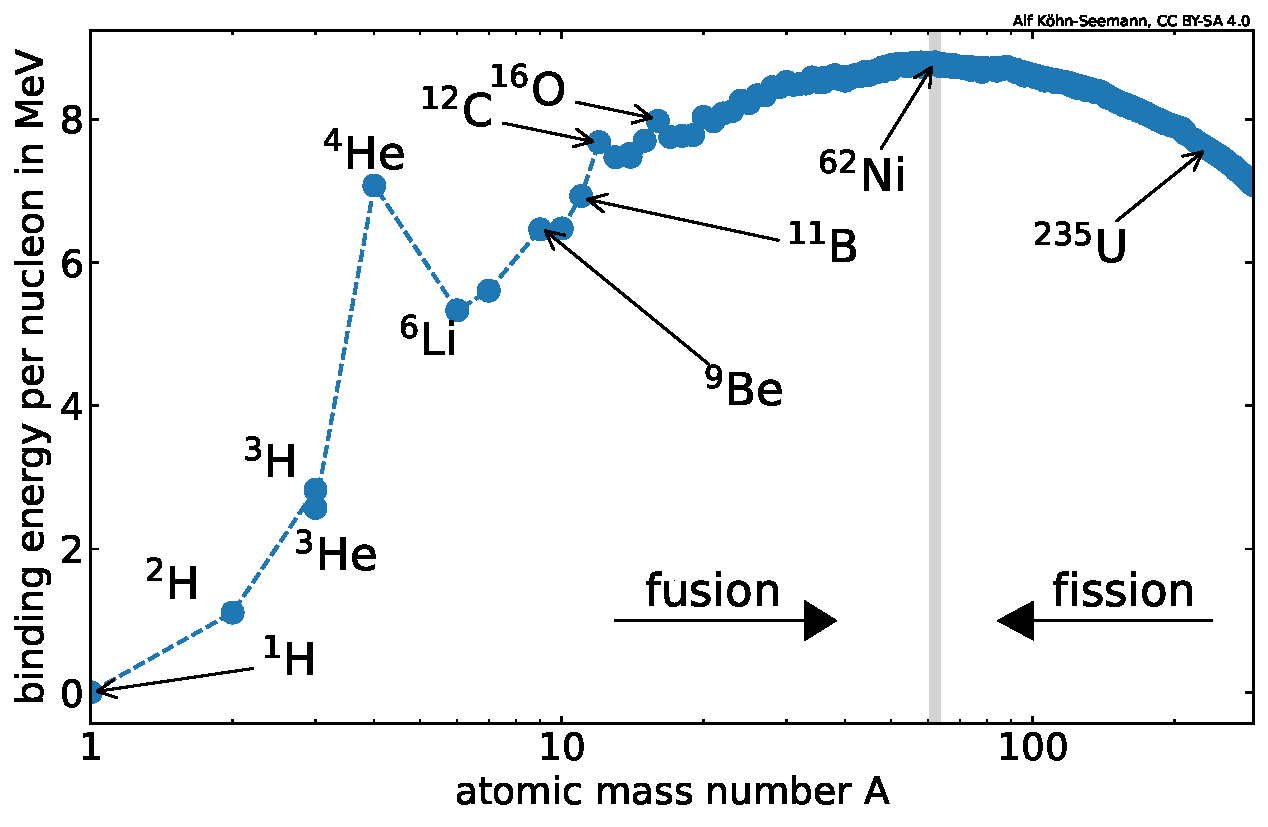
\includegraphics[width=\linewidth]{Figures/Chapter1/binding_energy_per_nucleon.pdf}
    \caption{Binding energy per nucleon \cite{kohn-seemann_alfkoehnfusion_plots_2021}.}
    \labfig{binding energy per nucleon}
\end{figure}

Nuclei are positively charged.
To be able to fuse, they must overcome the Coulomb barrier induced by the electromagnetic repulsion (see \reffig{potential energy diagram fusion}).
This Coulomb barrier increases with the charge of the nuclei (i.e.\ the number of protons).
This means that the nuclei must collide with a high enough velocity.
At the atomistic scale, the velocity $v_\mathrm{th}$ is a function of temperature (see \refeq{thermal velocity}).
This is one of the reasons why the probability of a fusion reaction (called cross-section) is temperature dependent.

\begin{equation}
    v_\mathrm{th} = \sqrt{\frac{k_B T}{m}}
    \labeq{thermal velocity}
\end{equation}
where $k_B = \SI{1.3806e-23}{m^2.s^{-2}.kg.K^{-1}}$ is the Boltzmann constant, $T$ is the nucleus temperature in \si{K} and $m$ is the nucleus mass in \si{kg}.


\begin{figure} [h]
    \centering
    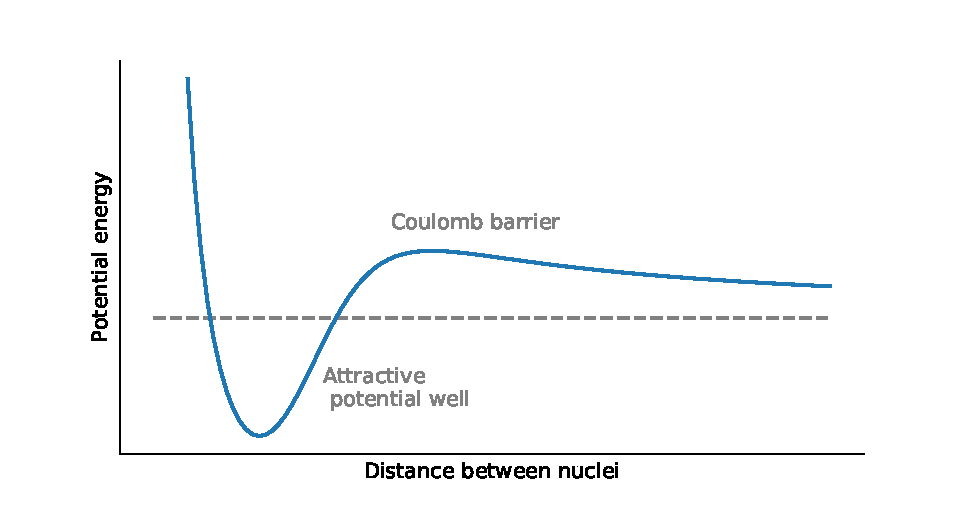
\includegraphics[width=\linewidth]{Figures/Chapter1/potential_energy.pdf}
    \caption{Evolution of the potential energy of two nuclei with their relative distance. Reproduced from \cite{mccracken_fusion_2013}.}
    \labfig{potential energy diagram fusion}
\end{figure}

Hydrogen, as the lightest element, has the lowest fusion temperature.
It is also the most abundant element on Earth (although bond to other elements).
Depending on which hydrogen \gls{isotope} is used, different fusion reactions are possible (see Equations \refeq{fusion reactions}) \cite{forrest_fendl-3_2012}.

\begin{subequations}
    \begin{equation}
         \ce{^2H + ^2H -> ^3H (\SI{1.01}{MeV}) + n (\SI{3.02}{MeV})}
    \end{equation}
    \begin{equation}
        \ce{^2H + ^2H -> ^3He (\SI{0.82}{MeV}) + n (\SI{2.45}{MeV})}
    \end{equation}
    \begin{equation}
        \ce{^2H + ^3H -> ^4He (\SI{3.5}{MeV}) + n (\SI{14.1}{MeV})}
    \end{equation}
    \begin{equation}
        \ce{^2H + ^3He -> ^4He (\SI{3.6}{MeV}) + p (\SI{14.7}{MeV})}
    \end{equation}
    \labeq{fusion reactions}
\end{subequations}

\begin{figure} [h]
    \centering
    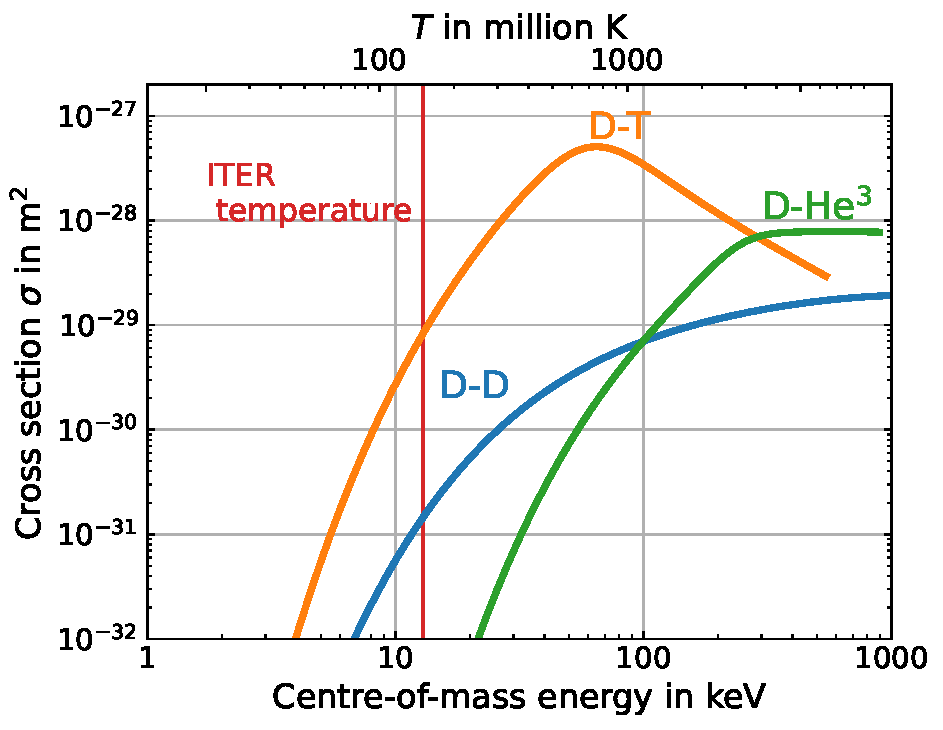
\includegraphics[width=\linewidth]{Figures/Chapter1/cross_sections_vs_temperature__Bosch.pdf}
    \caption{Fusion cross sections \cite{forrest_fendl-3_2012}.}
    \labfig{fusion cross sections}
\end{figure}
Each of these reactions has a different cross-section (measure of the reaction probability).
The \gls{D}-\gls{T} reaction is the one with the highest cross-section at `low` temperature (see \reffig{fusion cross sections}).
This is the reason why this reaction has been the focus of nuclear fusion for decades.
More recently, private companies have started experimenting with more exotic reactions like proton-boron (TAE Technologies) or $^2$H-$^3$He (Helion Energy).

% \begin{figure} [h]
%     \centering
%     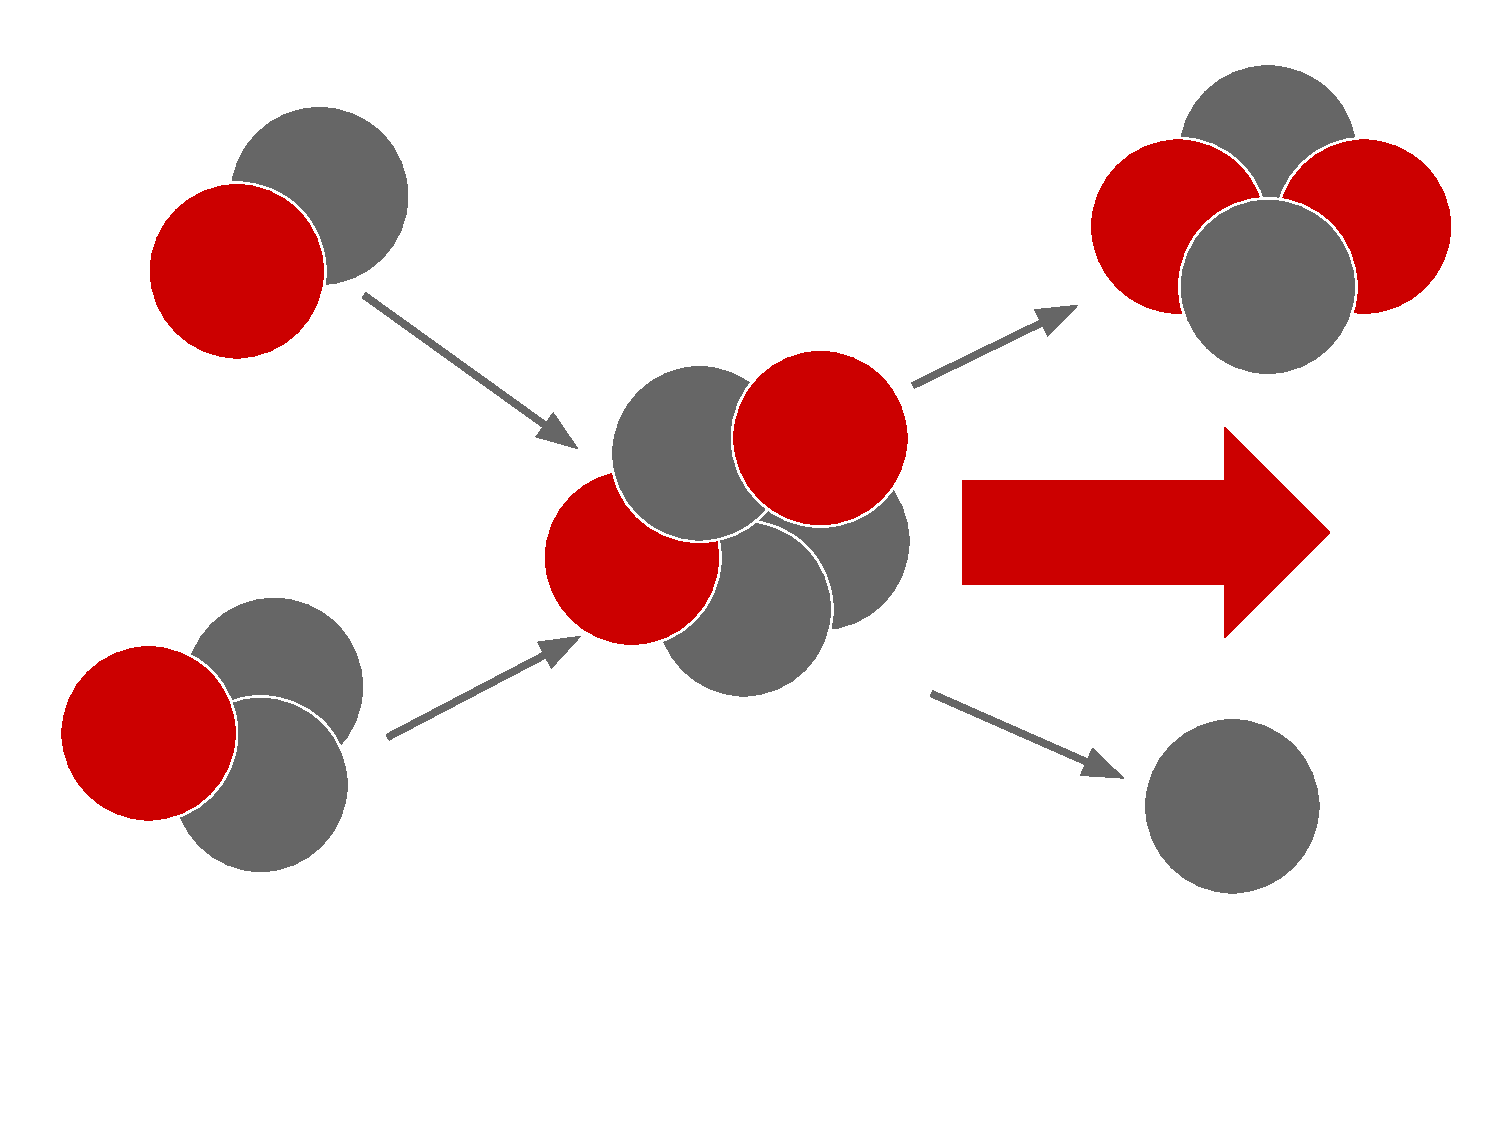
\includegraphics[width=\linewidth]{Figures/Chapter1/nuc_fus.pdf}
%     \caption{DT reaction}
% \end{figure}

\section{Tokamaks: how to bottle a star}

\subsection{Technology \cite{mccracken_fusion_2013}}
As explained above, for fusion to occur, the fuel must be heated up to millions of degrees.
A these temperatures, the DT gas becomes a \gls{plasma} where electrons are torn out from the nuclei.
The principle of magnetic confinement reactors is to trap the electrically charged particles in a magnetic cage.
The electrons and ions then gyrate around the magnetic field lines and the Larmor radius of the gyration is given by:
\begin{equation}
    R =  \frac{\sqrt{2 m T}}{e B}
\end{equation}
where $m$ is the mass of the particle, $T$ its temperature, $e$ its charge and $B$ the magnetic field.
In a hot \gls{plasma} (\SI{10}{keV}) with a strong magnetic field of \SI{3}{T}, the Larmor radius of ions is $\approx \SI{1}{mm}$, which is much smaller compared to the size of a reactor.
The Larmor radius of an electron is orders of magnitude smaller due to its lower mass.
Straight magnetic lines can therefore confine charged particles in the direction perpendicular to the field lines.
However, the particles are not confined in the parallel direction.

This issue can be solved by closing the field lines, forming a torus-shaped magnetic field.
However, this configuration poses another problem: bending the field lines creates a magnetic field gradient in the radial direction.
This magnetic field gradient and the centrifugal force cause the particles to drift upwards (or downwards depending on their charge).
Due to this drift, the particles end up escaping the magnetic confinement until they touch the walls of the chamber and neutralise (making it impossible for them to fuse).

Two options exist to compensate this drift.
The first is to add a poloidal component to the magnetic field and twist the magnetic lines.
This is done by inducting a current in the \gls{plasma} thanks to a central solenoid (see \reffig{tokamak magnetic field}).
This configuration is called \Gls{tokamak} which stands for `toroidalnaia kamera s magnitnymi katouchkami` (toroidal chamber with magnetic coils).

\begin{figure}[h]
    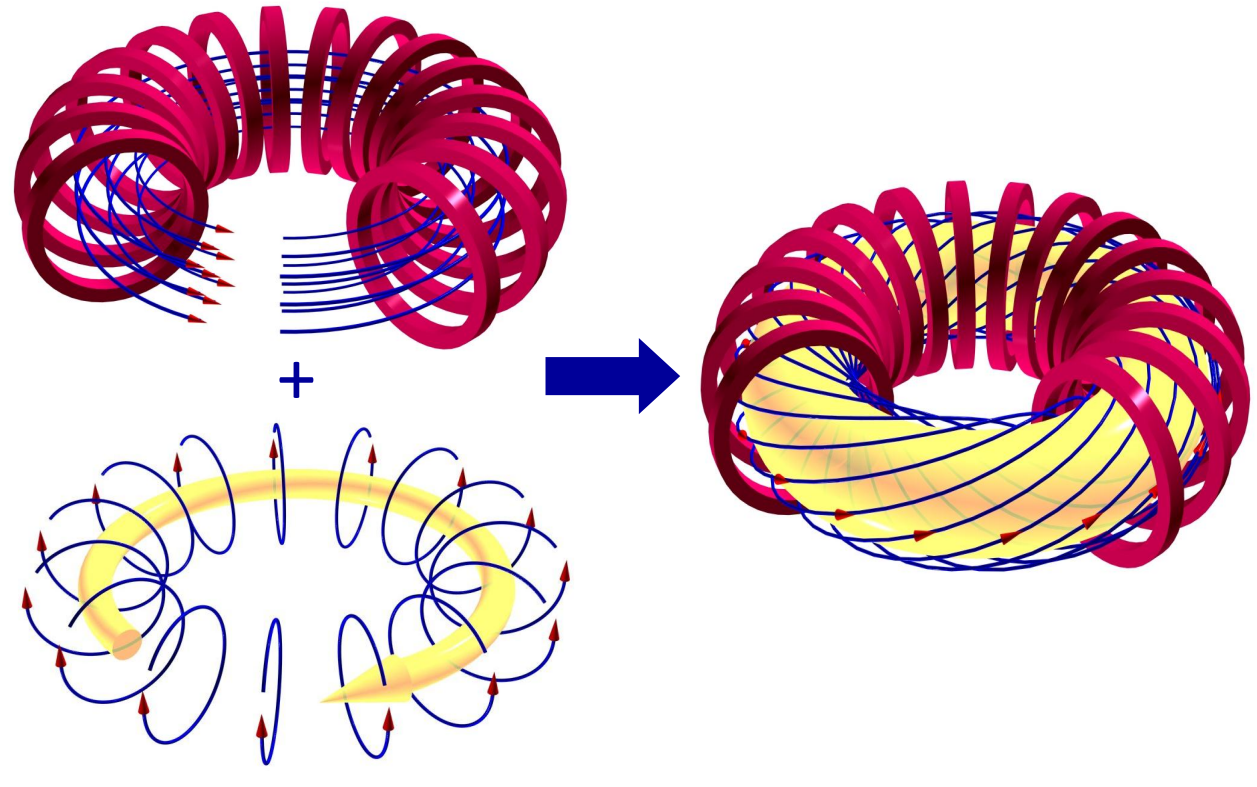
\includegraphics[width=\linewidth]{Figures/Chapter1/tokamak_magnetic_fields.png}
    \caption{Magnetic field lines in a tokamak. Contribution of the toroidal and poloidal components.}
    \labfig{tokamak magnetic field}
\end{figure}

The second option is to twist the magnetic field by twisting the toroidal coils themselves.
This configuration is called a \gls{stellarator} and has the advantage of not having an induced current and is therefore inherently steady-state.
The \gls{tokamak}, on the other hand, is a pulsed device.
This is because the central solenoid has a limited capacity.
The main drawback of the \gls{stellarator} is the complexity of the coils.
Since each coil has a unique shape, the cost of manufacturing such a reactor is higher than \glspl{tokamak} for which coils can be manufactured in series.

\subsection{Triple product}
The power balance in a fusion reactor is given by \cite{mccracken_fusion_2013}:
\begin{equation}
    \frac{\partial W}{\partial t} = P_\mathrm{fusion} + P_\mathrm{heating} - P_\mathrm{losses}
    \labeq{plasma energy balance}
\end{equation}
$W$ is the thermal energy density stored in the \gls{plasma} and can be expressed in \si{J.m^{-3}} by:
\begin{equation}
    W = 3 n T
\end{equation}
where $n$ is the \gls{plasma} density in \si{m^{-3}} and $T$ is the \gls{plasma} temperature in \si{J}.
$P_\mathrm{fusion}$, expressed in \si{W.m^{-3}}, is the power density generated from fusion reactions themselves and can be expressed by:
\begin{equation}
    P_\mathrm{fusion} = n_D n_T \left\langle \sigma \right\rangle E
\end{equation}
where $n_D$ and $n_T$ are the densities in \si{m^{-3}} of deuterium and tritium respectively, $\left\langle \sigma \right\rangle$ is the DT reactivity in \si{m^3.s^{-1}} and $E$ is the energy of the fusion reaction in \si{J}.
Because the neutrons have little interaction with the \gls{plasma}, $E \approx E_\alpha = \SI{3.56}{MeV}$.
Moreover, assuming a 50\%-50\% mixture of deuterium and tritium, $n_D = n_T = \frac{1}{2} n$.
The fusion power can therefore be written as:
\begin{equation}
    P_\mathrm{fusion} = \frac{1}{4} n^2 \left\langle \sigma \right\rangle E_\alpha
\end{equation}

The amplification factor $Q$ defines the ratio of the fusion power by the heating power.
The heating power $P_\mathrm{heating}$ is therefore written as:
\begin{equation}
    P_\mathrm{heating} = \frac{P_\mathrm{fusion}}{Q}
\end{equation}

Finally, $P_\mathrm{losses}$ is the rate at which the \gls{plasma} loses energy, either by losing mass (particles escaping the magnetic cage) or by radiation.
It is characterised by an energy confinement time $\tau_E$ and can be expressed as:
\begin{equation}
    P_\mathrm{losses} = \frac{W}{\tau_E} = \frac{3 n T}{\tau_E}
\end{equation}

Assuming energy equilibrium (i.e.\ $\frac{\partial W}{\partial t} = 0$), \refeq{plasma energy balance} can therefore be written as:
\begin{align}
    P_\mathrm{losses} &= P_\mathrm{fusion} + P_\mathrm{heating} \\
    \Leftrightarrow \frac{3 n T}{\tau_E} &= \frac{1}{4} n^2 \left\langle \sigma \right\rangle E_\alpha + \frac{P_\mathrm{fusion}}{Q}
\end{align}

Re-arranging the terms, one can obtain:
\begin{equation}
    n T \tau_E = \frac{12 T^2}{\left\langle \sigma \right\rangle E_\alpha} \cdot \frac{1}{1 + \frac{1}{Q}}
    \labeq{triple product}
\end{equation}

$n T \tau_E$ is known as the \textit{triple product}, a figure of merit describing the performance of a fusion reactor.
\refeq{triple product} gives the triple-product required to achieve a given amplification factor $Q$ at a given temperature $T$.

When $P_\mathrm{heating}$ approaches zero (i.e.\ the auxiliary heating systems are shut down), the amplification factor $Q$ approaches $\infty$.
Therefore:
\begin{equation}
    n T \tau_E \rightarrow \frac{12 T^2}{\left\langle \sigma \right\rangle E_\alpha}
    \labeq{triple product infinity}
\end{equation}

The quantity $T^2/\langle \sigma \rangle$ has a minimum around $T=\SI{14}{keV}$.
Furthermore, when $\SI{10}{keV} < T < \SI{20}{keV}$, the DT reactivity can be approximated by $\langle \sigma \rangle \approx 1.1 \times 10^{-24} T^2$.

\refeq{triple product infinity} can therefore be written as:
\begin{equation}
    n T \tau_E \geq \SI{3e21}{keV.s.m^{-3}}
\end{equation}

This is known as the Lawson criterion, which needs to be satisfied in order to reach \textit{ignition} ($Q = \infty$).


Fusion devices can therefore be classified into three categories.
Stars like our Sun have very high confinement times and densities while remaining at relatively low temperatures (the sun core is at \SI{1.2}{keV}).
Magnetic confinement devices (\glspl{tokamak}, \glspl{stellarator}, etc.) exhibit temperatures orders of magnitude higher than stars but have confinement times of the order of $\sim \SI{1}{s}$.
A third way of achieving fusion is to heat and compress a target of fuel with either lasers (\acrshort{nif} \sidecite{zylstra_burning_2022}, Laser Mega Joule \sidecite{miquel_laser_2016}), pistons (General Fusion) or by smashing it at high speed with a projectile (First Light Fusion).
These devices, known as \textit{inertial fusion devices}, exhibit extremely high densities ($\sim \SI{e31}{m^{-3}}$) but short confinement times ($\sim \SI{e-11}{s}$).
 
So far, no fusion device has been able to even reach \textit{break-even} ($Q = 1$) (see \reffig{triple product vs T}).
The record of $Q = 0.68$ by the European \gls{tokamak} \gls{jet} and was performed in 1997 \sidecite{mailloux_overview_2022}.
The objective of the \gls{iter} \gls{tokamak}, currently under construction in France, is to demonstrate an amplification factor of $Q=10$ over \SI{400}{s} \sidecite{casper_development_2013}. 
Note that \acrshort{iter} will not produce any electricity as this will be the role of a future fusion reactor: DEMO \sidecite{federici_overview_2014}.
Other designs aim at demonstrating \gls{plasma} gain (i.e.\ $Q > 1$) sooner than \acrshort{iter} and at a smaller scale (see \reffig{comparison reactors}).
This is the case of \acrshort{sparc} and \acrshort{arc} developed by Commonwealth Fusion Systems and MIT \sidecite{sorbom_arc_2015,creely_overview_2020} or \acrshort{step} designed by the \gls{ukaea} \sidecite{wilson_steppathway_2020}.

\begin{figure}
    \centering
    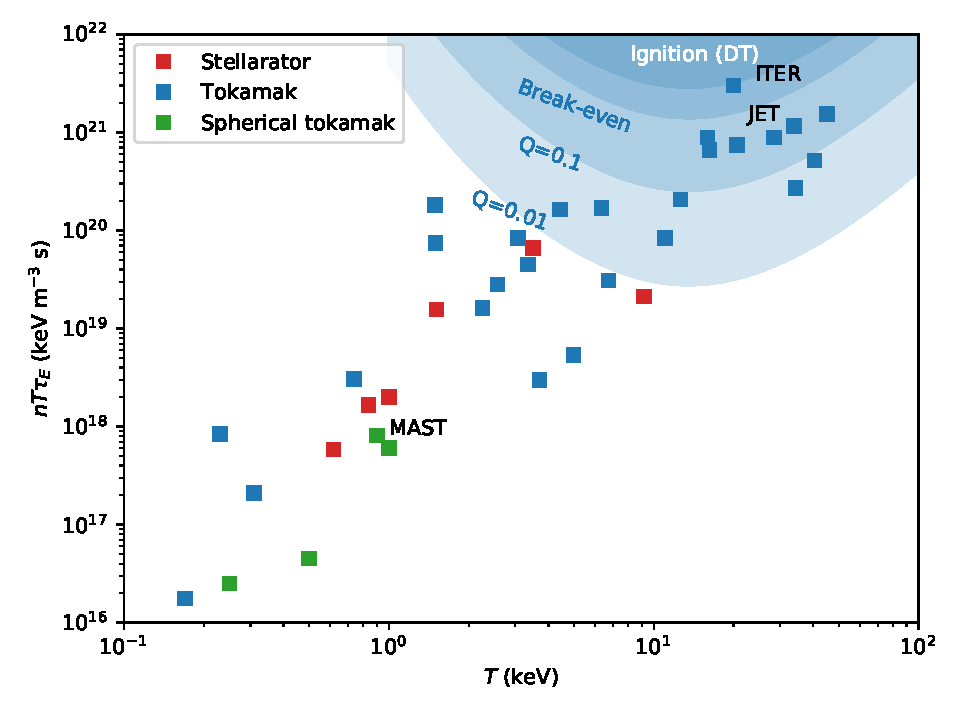
\includegraphics[width=\linewidth]{Figures/Chapter1/triple_product_vs_T.pdf}
    \caption{Triple product. An interactive version of this plot is available at \cite{delaporte-mathurin_remdelaportemathurinfusion-world_2022}.}
    \labfig{triple product vs T}
\end{figure}

\begin{figure}
    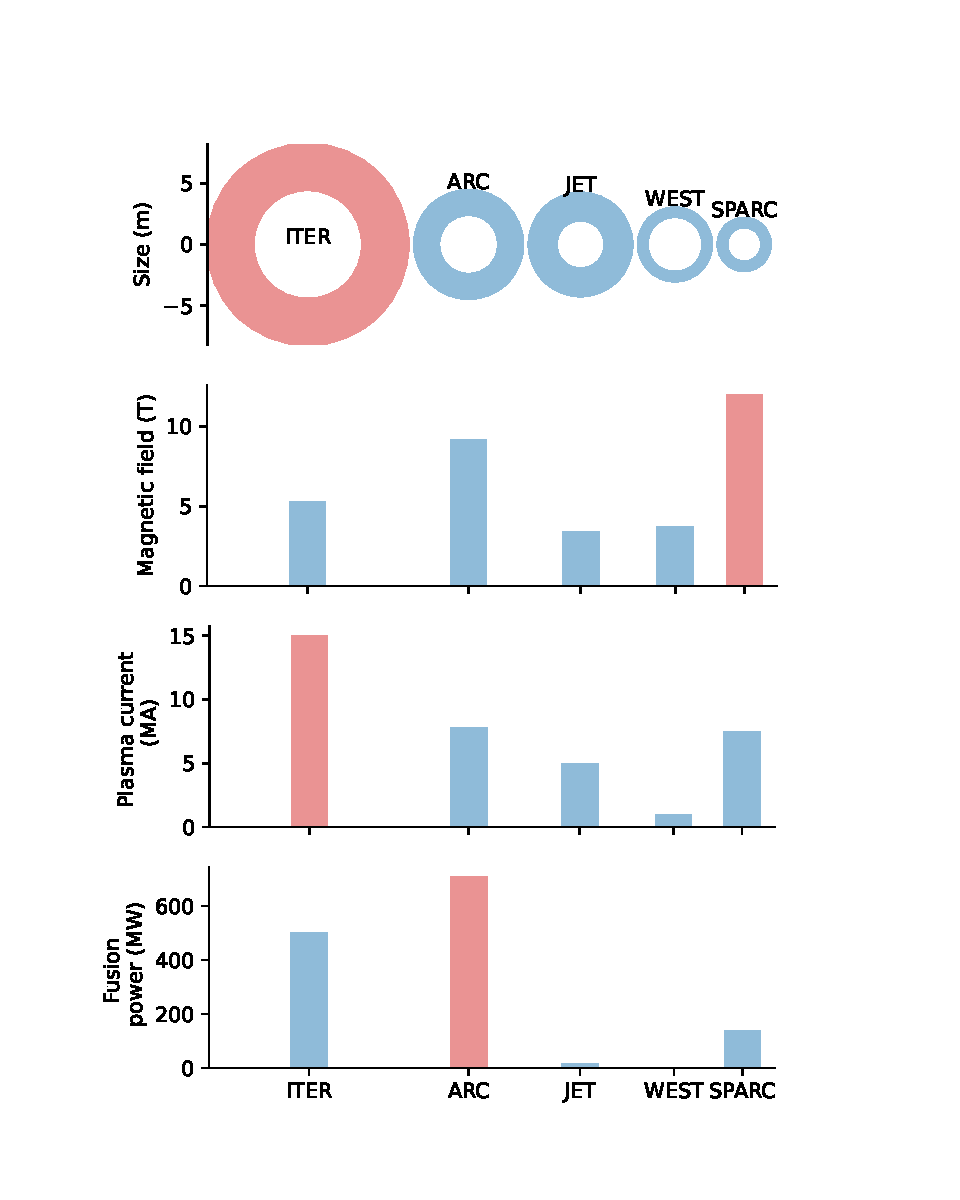
\includegraphics[width=0.9\linewidth]{Figures/Chapter1/comparison_reactors.pdf}
    \caption{Comparison of the tokamaks \acrshort{iter}, JET, ARC, WEST and SPARC. Data from \cite{delaporte-mathurin_remdelaportemathurinfusion-world_2022}.}
    \labfig{comparison reactors}
\end{figure}

\subsection{Plasma-facing materials}

The walls of a fusion reactor are exposed to intense heat and particle fluxes.
The choice of \glspl{pfm} is therefore crucial.

An appropriate \gls{pfm} must have good thermal properties to withstand the extreme heat fluxes.
To minimise electric arcs, the materials must have a high electrical conductivity.
A high thermal conductivity is required as well as a very high melting point to enhance heat exhaust but also minimise the impact of arcing (material release from erosion) \sidecite{ivanova_plasma-facing_2012, mccracken_review_1980}.
The material must also resist to thermal shock encountered during short \gls{plasma} discharges or transient events in the \gls{plasma} \sidecite{van_den_kerkhof_impact_2021}.

In order to maximise the components' lifespan, \glspl{pfm} must resist erosion.
This is even more important when the eroded particle reduce \gls{plasma} performances by making it radiate and cool down.

The choice of a \gls{pfm} is also critical from the nuclear safety point of view.
First, the quantity of tritium retained in the materials need to be minimised (this point will be detailed in \refsec{the tritium issue}).
Second, neutron activation of the material can increase the quantity of radioactive waste and must be minimised.

One of the first \gls{pfm} was \gls{cfc} \sidecite{linke_challenges_2019}.
\gls{cfc} had the great advantage of not melting and withstand very high heat fluxes.
Using \gls{cfc} also increased the \gls{plasma} performances greatly \sidecite{federici_plasma-material_2001}.
Unfortunately, graphite being porous, hydrogen (and therefore tritium) retention was high \sidecite{sugiyama_measurement_2004}.
Plus carbon can react with \gls{plasma} particles forming methane.
Methane is then deposited on locations hard to access in the reactor \gls{trapping} tritium even more.
For these two safety reasons, \gls{cfc} was replaced with \Gls{W} or \gls{Be} (or both).
The advantage of \gls{Be} is that it creates a stable oxide.
The formation of this oxide layer consumes oxygen and reduces the oxygen level in the plasma.

\Gls{W} has a very high melting point (\SI{3422}{\celsius}) and retains less tritium \sidecite{pajuste_tritium_2021}.
However, \Gls{W} being a high-Z element, eroded \Gls{W} will make the \gls{plasma} radiate and cool it down.
For this reason, the \acrshort{iter} divertor will be made of \Gls{W} but the first wall (which has a large surface area) will be made of \gls{Be}.

\subsection{Divertor}\labsec{divertor section}

In a fusion reactor, heat and particles (fusion ashes) need to be extracted.
In most \glspl{tokamak}, the escaping \gls{plasma} is diverted towards a dedicated component that is heat-resistant.
Such a configuration is called a \emph{\gls{divertor}} configuration.
The \gls{divertor} allows the creation of a \gls{x-point} and a \gls{separatrix} decoupling the \gls{plasma} edge from the walls. 
The X-divertor is a common configuration (used in \acrshort{asdex}, \acrshort{west}, \acrshort{jet}, \acrshort{iter}) but more advanced configurations exist such as the Super-X \gls{divertor} (\acrshort{mast-u}) \sidecite{havlickova_effect_2015}, X-Point Target (\acrshort{sparc}) \sidecite{rodriguez-fernandez_overview_2022, kuang_divertor_2020} or the Snowflake configurations \sidecite{ryutov_snowflake_2015}.

\begin{figure} [h]
    \centering
    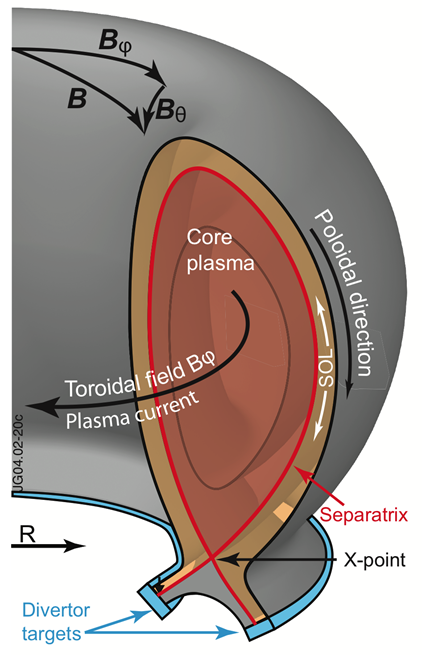
\includegraphics[width=0.5\linewidth]{Figures/Chapter1/sketch_divertor.png}
    \caption{Sketch of the tokamak divertor configuration (source: EFDA-JET).}
    \labfig{divertor diagram}
\end{figure}

In a \gls{divertor} configuration, the intersection between the magnetic field lines and the targets are called \emph{\glspl{strike point}}.
The X-divertor has two \glspl{strike point} on the inner and outer targets (see \reffig{divertor diagram}).
At these \glspl{strike point}, the targets will experience very intense heat and particle fluxes (see \reffig{divertor exposure conditions}).

\begin{figure} [h]
    \centering
    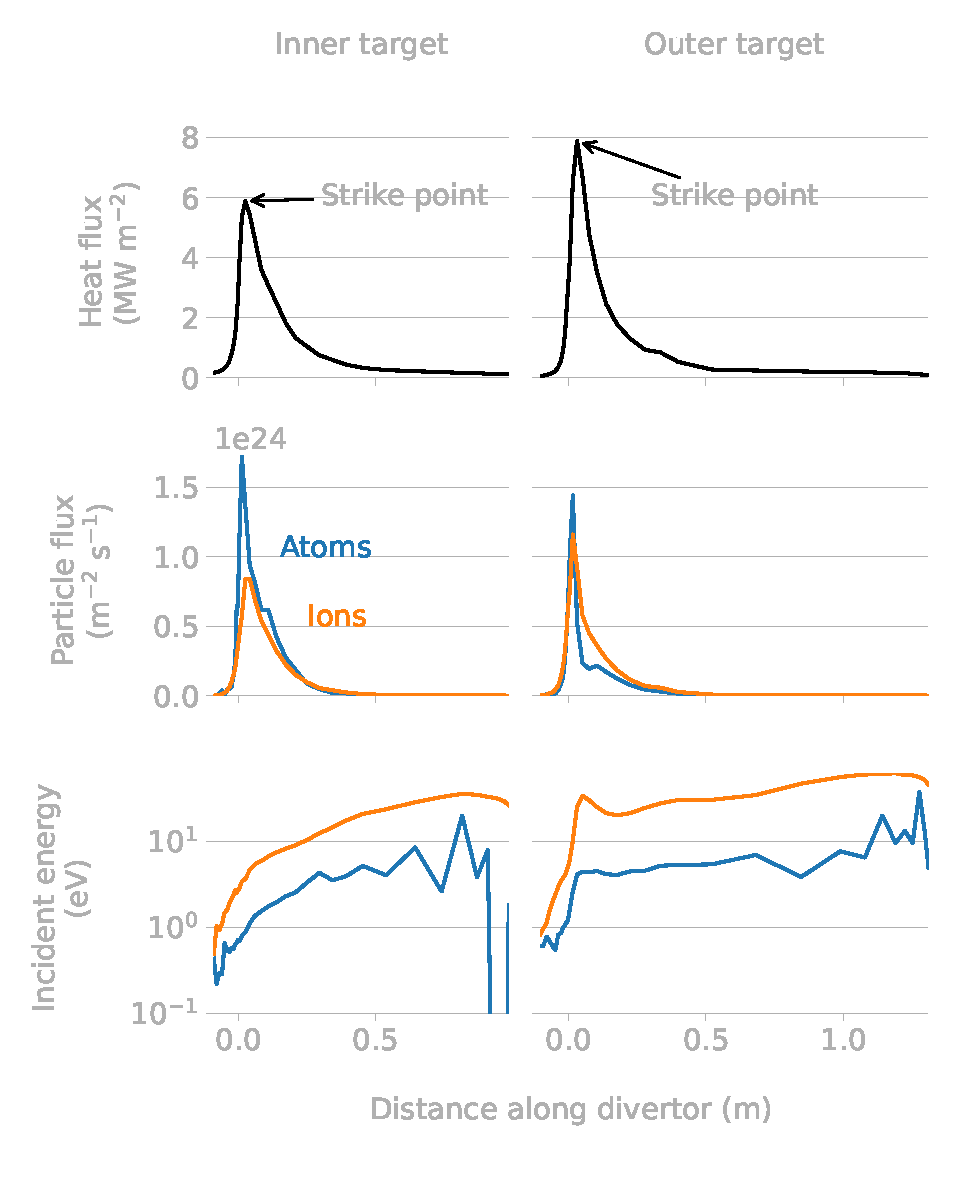
\includegraphics[width=\linewidth]{Figures/Chapter1/divertor_exposure_conditions.pdf}
    \caption{Heat flux, particle flux and particle energy along the \acrshort{iter} divertor computed by the edge-plasma simulation code SOLPS (shot \#122399) \cite{pitts_physics_2019}.}
    \labfig{divertor exposure conditions}
\end{figure}

The \acrshort{iter} divertor will be composed of 54 cassettes (see \reffig{monoblock to divertor}).
Each cassette is made of two targets - the \gls{ivt} and \gls{ovt} -, a dome and two reflector plates.
The inner and outer \glspl{strike point} (respectively \acrshort{isp} and \acrshort{osp}) will be located on the \gls{ivt} and the \gls{ovt}.
% A prototype of the \gls{ivt} is shown on \reffig{inner target photo}.
These elements are themselves made of rows, called \glspl{pfuLabel}, of small unit bricks of a few dozens of millimetres called \glspl{monoblock}.
In \acrshort{iter}, the \gls{ivt} has 16 \glspl{pfuLabel} and the \gls{ovt} has 22 \glspl{pfuLabel}.
\Glspl{monoblock} are typically made of a \Gls{W} substrate with a cooling pipe running through.
This cooling channel is necessary to keep the component's temperature below its operating limit and exhaust heat.

Several \gls{monoblock} designs are currently studied for DEMO with varying dimensions, different materials for the cooling pipe or the interlayer, etc. \sidecite{vizvary_european_2020, huang_tungsten_2016, hirai_use_2016, domptail_design_2020}.
The main candidate is the ITER-like design, the type of \gls{monoblock} that will be used in \acrshort{iter} \cite{hirai_use_2016}.
This design has a tungsten substrate with a CuCrZr cooling pipe and a Cu interlayer for compliance.
In \acrshort{iter}, \glspl{monoblock} will be \SI{12}{mm}-thick whereas they will be thinner (\SI{4}{mm}) in DEMO \sidecite{you_european_2018}.

\begin{figure*}
    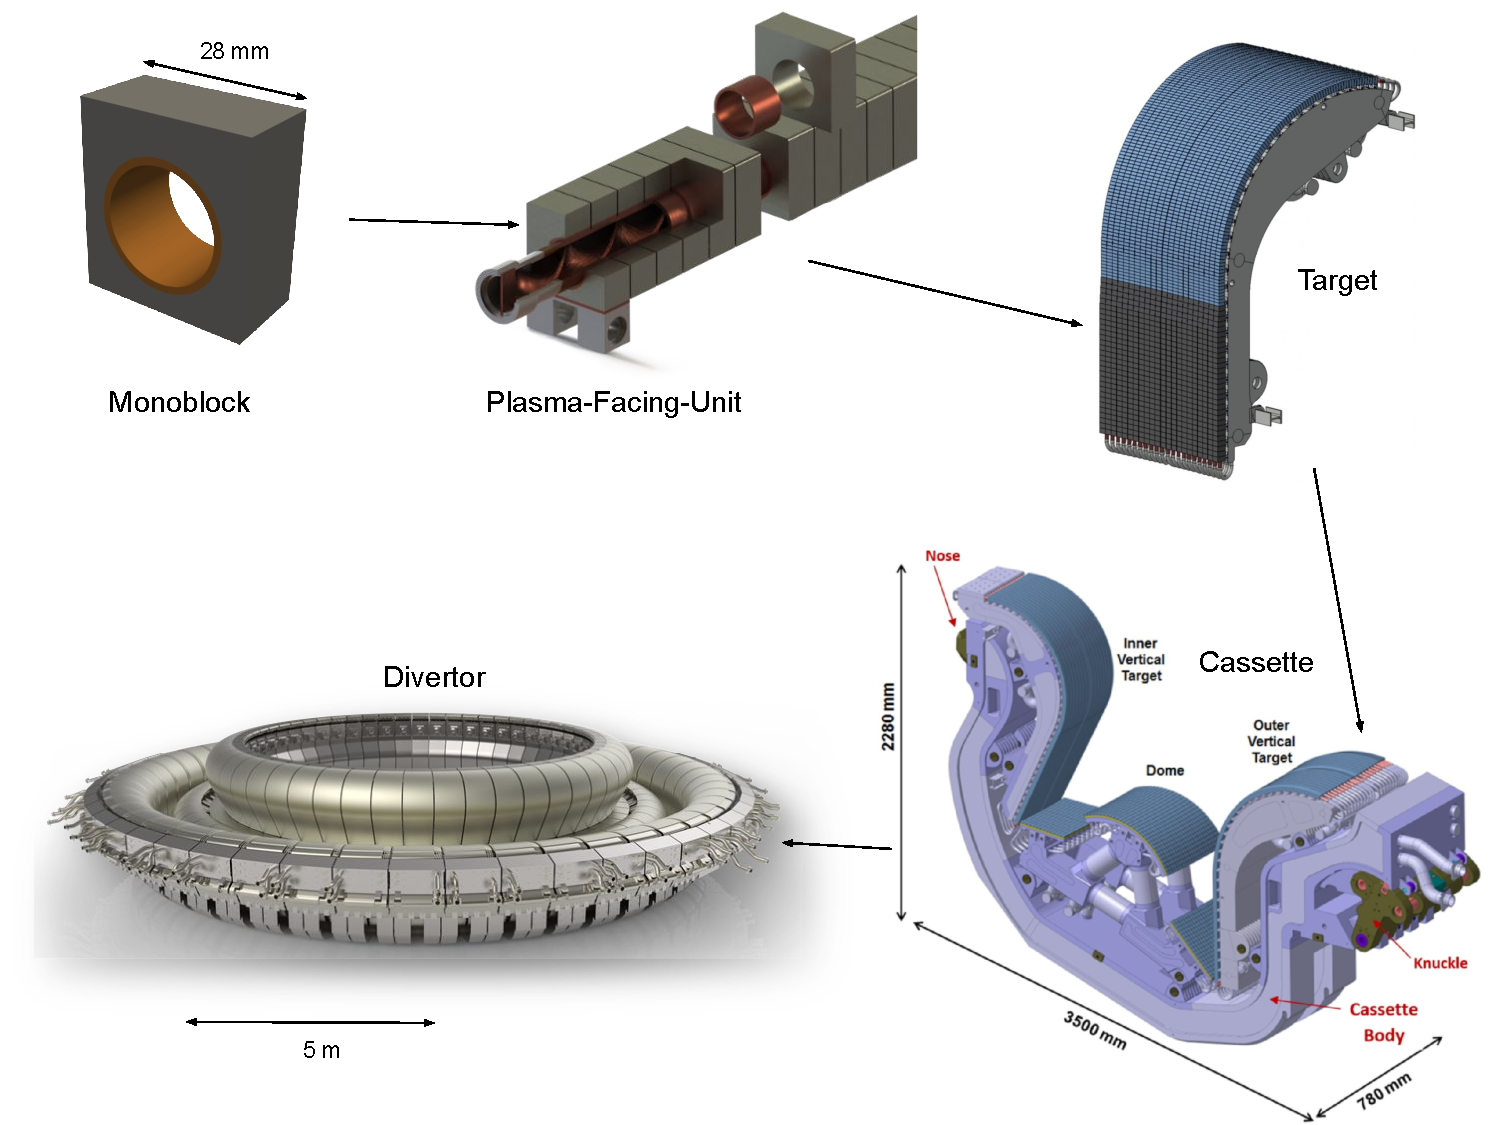
\includegraphics[width=\linewidth]{Figures/Chapter1/monoblock_to_divertor.pdf}
    \caption{Structure of the \acrshort{iter} divertor. (images: ITER Organization, \cite{guerrini_fabrication_2021}).}
    \labfig{monoblock to divertor}
\end{figure*}

% \begin{figure} [h]
%     \centering
%     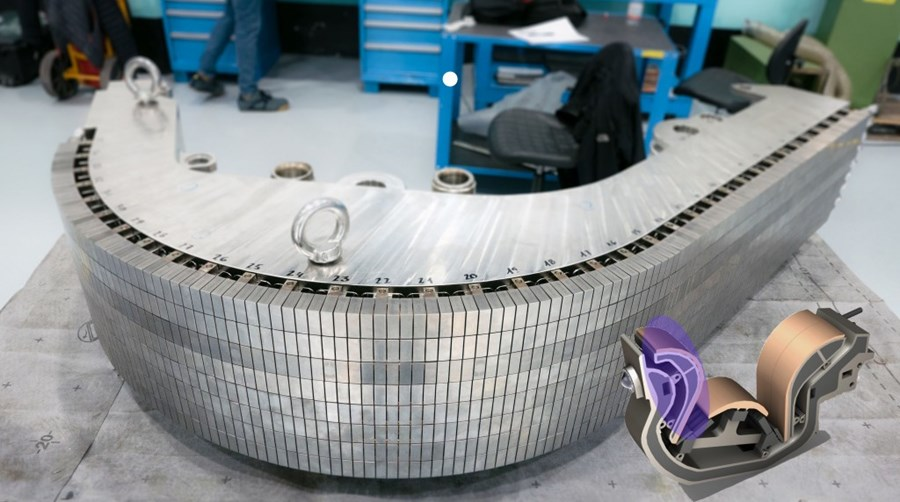
\includegraphics[width=0.8\linewidth]{Figures/Chapter1/inner_target_iter.jpg}
%     \caption{Prototype of the inner vertical target (source: ITER Organization).}
%     \labfig{inner target photo}
% \end{figure}

Studies on ITER-like \glspl{monoblock} have demonstrated the resistance of the \gls{monoblock} design to high heat loads while investigating the effect of \Gls{W} recrystallisation \sidecite{durif_impact_2019, durif_modelisation_2019, visca_manufacturing_2018} (see \reffig{monoblock_temperature_exp_model}).

\begin{figure} [h]
    \centering
    \begin{subfigure}[t]{0.45\linewidth}
            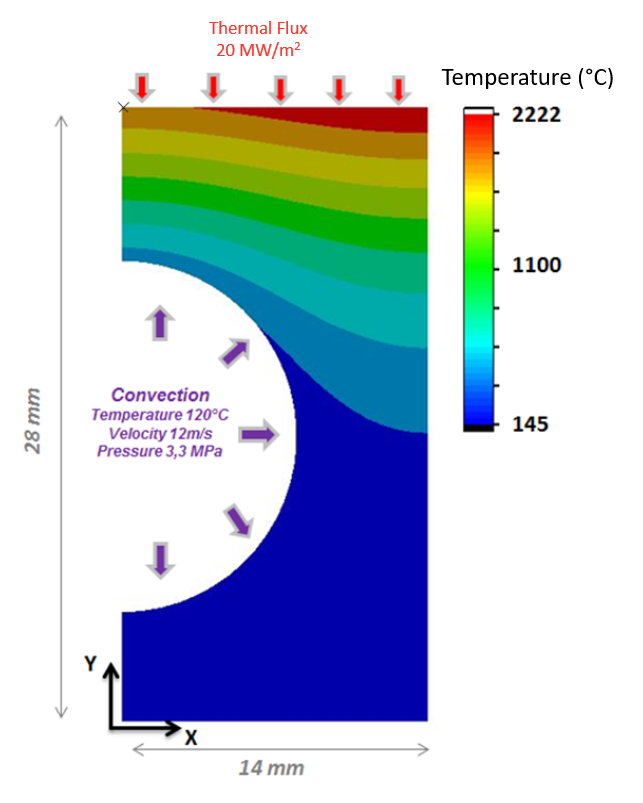
\includegraphics[width=\linewidth]{Figures/Chapter1/alan_durif_monoblock.png}
            \caption{Simulated temperature field in a monoblock at \SI{20}{MW.m ^{-2}} heat loading, water cooling at \SI{120}{\celsius}. Reproduced from \cite{durif_modelisation_2019}.}
    \end{subfigure}\hfill%%
    \begin{subfigure}[t]{0.45\linewidth}
            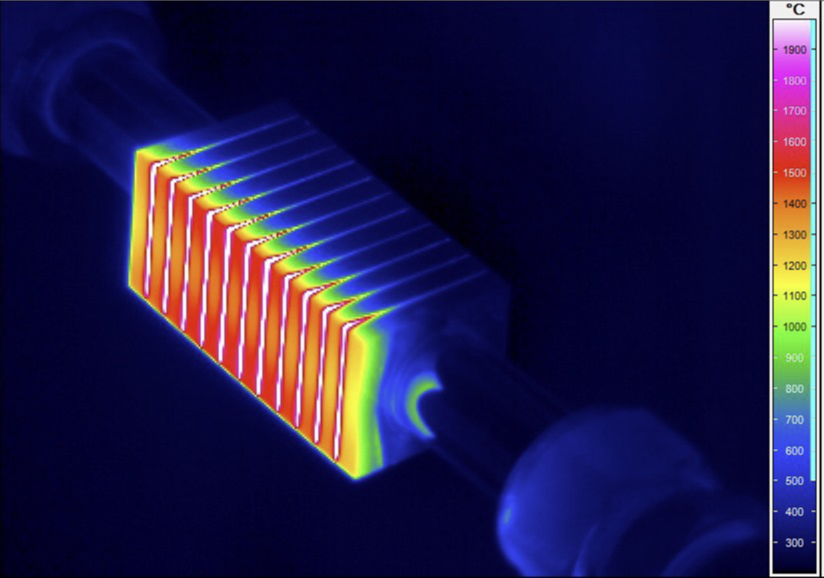
\includegraphics[width=\linewidth]{Figures/Chapter1/monoblock_experimental_temperature_field.png}
            \caption{Experimental measurement of monoblocks thermal response at \SI{20}{MW.m ^{-2}} heat loading, water cooling at \SI{130}{\celsius}. Reproduced from \cite{visca_manufacturing_2018}.}
    \end{subfigure}
    \caption{Thermal response of ITER-like monoblocks.}
    \labfig{monoblock_temperature_exp_model}
\end{figure}

\section{The tritium issue} \labsec{the tritium issue}

Tritium is a radioactive \gls{isotope} of hydrogen with a half-life is 12.32 years \sidecite{jordan_half-life_1967}.
It decays into $^3$He emitting a beta particle (see \refeq{tritium decay}).

\begin{equation}
    \ce{^3H -> ^3He + e^- (\SI{18.590}{keV})}
    \labeq{tritium decay}
\end{equation}

This is an issue for both the fuel supply chain and nuclear safety.

\subsection{Breeding}
Due to its radioactive nature, tritium is very rare on Earth.
The current reserve of tritium in the world is a few dozens of kilograms.
It is naturally produced by interaction of cosmic rays with the nitrogen in the atmosphere (\SI{0.2}{kg} per year).
Tritium is however produced in larger quantities in fission \gls{candu} reactors as a by-product (\SI{130}{g} per year per \gls{candu} reactor \sidecite{ni_tritium_2013}).

\acrshort{iter} itself will consume around \SI{18}{kg} of tritium over the duration of its operation \sidecite{glugla_iter_2007}, which represent a yearly consumption of \SI{0.9}{kg} for a 20-year lifetime.
A \SI{800}{MWe} DEMO-type commercial fusion reactor would burn around \SI{300}{g} of tritium per day ($\approx \SI{100}{kg}$ a year).

For all these reasons, tritium must be produced on-site in large quantities for a fusion economy to be possible.

To this end, the neutrons of the DT fusion reactions will be harnessed in a component containing \gls{Li} surrounding the \gls{plasma} called the \emph{\gls{breeding blanket}} (see \reffig{blanket_shimwell}).


\begin{figure}
    \centering
    \begin{subfigure}{0.45\linewidth}
        \includegraphics{Figures/Chapter1/blanket_shimwell_top_view.png}
        \caption{View from above.}
    \end{subfigure}%
    \qquad
    \begin{subfigure}{0.45\linewidth}
        \includegraphics{Figures/Chapter1/blanket_shimwell_side_view.png}
        \caption{Side view.}
    \end{subfigure}
    \caption{DEMO model showing HCLL blankets \cruleme[lithiumgreen]{0.3cm}{0.3cm}, plasma \cruleme[plasmapink]{0.3cm}{0.3cm}, magnets \cruleme[magnetred]{0.3cm}{0.3cm}, and structural steel \cruleme[steelgray]{0.3cm}{0.3cm}. Reproduced from \cite{shimwell_multiphysics_2019}.}
    \labfig{blanket_shimwell}
\end{figure}

Depending on the \gls{Li} \gls{isotope}, two reactions can occur:

\begin{align}
    \text{n} + \text{\textsuperscript{6}Li}  \ \ &\xrightarrow{} \ \ \text{\textsuperscript{3}H} + \alpha + \SI{4.8}{MeV}\\
    \text{n} + \text{\textsuperscript{7}Li}  \ \ &\xrightarrow{} \ \ \text{\textsuperscript{3}H} + \alpha + \text{n}' - \SI{2.5}{MeV} 
\end{align}

Several \glspl{breeding blanket} designs have been proposed divided in three main categories: ceramic concepts, liquid metal concepts, and molten-salts concepts.
All designs differ in the choice of tritium breeder, coolant and geometry.

The European candidates for \glspl{breeding blanket} in DEMO are the \gls{wcll} \sidecite{aubert_design_2020, del_nevo_recent_2019}, the \gls{hcpb} \sidecite{hernandez_overview_2018, hernandez_new_2017,pereslavtsev_neutronic_2017}, the \gls{hcll} \sidecite{aubert_status_2018,jaboulay_nuclear_2017} and the \gls{dcll} \sidecite{urgorri_tritium_2017, palermo_neutronic_2015} \sidecite{federici_overview_2019}.

The \gls{tbr} is defined by the number of tritium atoms produced by generated neutrons.
In order to ensure tritium self-sufficiency, the \gls{tbr} of the blanket must be greater than or equal to one \sidecite{abdou_blanketfirst_2015}.
A \gls{tbr} greater than one can only be obtained by neutron multiplication with lead or \gls{Be}.

Moreover, the \gls{tbr} must account for:
\begin{itemize}
    \item losses via \gls{permeation}, \gls{trapping}, radioactive decay (5\% per year)
    \item safety reserve in case of interruption of the fuel cycle
    \item supply of new reactors, also called the \emph{\gls{startup inventory}}
\end{itemize}

The \gls{tbr} target in conventional power plants is around 1.05 \sidecite{shimwell_multiphysics_2019}.
Though this would achieve self-sufficiency, it is not enough to sustain the development of a fusion energy market.

% The desired doubling time of fusion power plants will drive this last point \sidecite{bockhoff_tritium_1983}.
The evolution of the maximum fusion power on the grid $P_\mathrm{max}$ can be expressed as:

\begin{equation}
    P_\mathrm{max} = P_\mathrm{plant} \times 2^{t/\tau_2}
\end{equation}
where $\tau_2$ is the doubling time (i.e.\ the time after which a plant has doubled its initial tritium \gls{inventory}), $t$ is the time, and $P_\mathrm{plant}$ is the power of a single plant.
This expression assumes the only source of tritium is the reactors currently under operation.

Assuming $P_\mathrm{plant} = \SI{1}{GW}$, with a doubling time $\tau_2 = \SI{2}{years}$, it will take \SI{20}{years} to produce \SI{1}{TW} of fusion electricity on the grid (see \reffig{fusion power doubling time}).
This time reaches \SI{50}{years} with a doubling time of \SI{5}{years}.

\begin{figure}
    \centering
    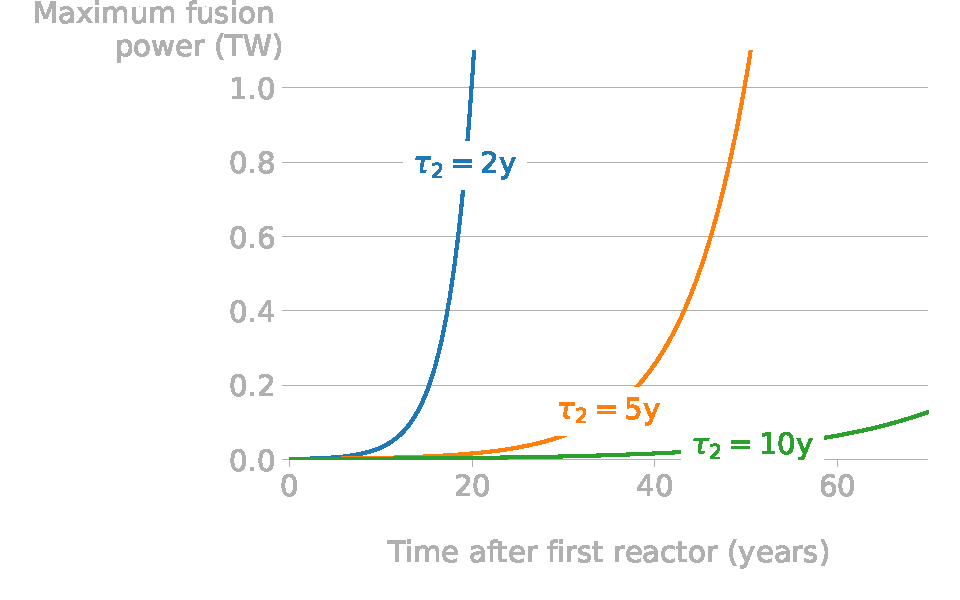
\includegraphics[width=0.8\linewidth]{Figures/Chapter1/doubling_time.pdf}
    \caption{Evolution of the maximum fusion power on the grid for different doubling times.}
    \labfig{fusion power doubling time}
\end{figure}

For fusion power plants to achieve a doubling time $\tau_2 \leq \SI{3}{years}$ (doubling times in power industry are typically \SI{5}{years}), the \gls{tbr} must be greater than 1.15 \sidecite{abdou_physics_2020}.
Other key parameters influence the required \gls{tbr} (for a given doubling time) like the tritium burn-up fraction, the fueling efficiency, the plant availability factor...

Tritium transport in \glspl{breeding blanket} is crucial as trapped tritium in solid parts would increase the \gls{startup inventory}.
For a given doubling time, a higher \gls{startup inventory} means a higher \gls{tbr} requirement.
The blanket \gls{inventory} in the solid parts can be reduced by (1) reducing the amount of solid components (this will also increase the \gls{tbr} \cite{shimwell_multiphysics_2019}) (2) designing permeation barriers \sidecite{utili_design_2022}.
% Understanding hydrogen transport in these components is therefore crucial for the future of nuclear fusion technology.

\subsection{Safety}
Tritium is also an issue in terms of nuclear safety.
As a radioactive \gls{isotope}, its ingestion - in the form of tritiated water HTO - is a health hazard.
Its biological half-life (i.e.\ once ingested by humans) is around 10 days - which can be considered as low toxicity \sidecite{bridges_review_2007,janssens_emerging_2007}.
Tritium's half-life once incorporated in organic compounds increases to 40 days and is associated with a higher toxicity \cite{bridges_review_2007}.
To put tritium toxicity in perspective, it has been estimated that drinking \SI{2}{L} of water with the highest permissible level of tritium contamination (\SI{10000}{Bq.L^{-1}}) each day for a year results in a total radiation dose of \SI{0.1}{mSv}, which is equivalent to two weeks natural radioactivity exposure \sidecite{hyatt_radioactive_2021}.

To limit the potential environmental releases due to a loss of vacuum accident, its \gls{inventory} in fusion reactors must be limited \sidecite{honda_analyses_2000}.
In \acrshort{iter} for instance, the in-vessel \gls{inventory} of tritium is limited to \SI{1}{kg} including \SI{120}{g} retained in cryo-pumps and \SI{180}{g} of measurement uncertainties \sidecite{roth_tritium_2008,de_temmerman_efficiency_2017}.
This limit has been determined to avoid evacuation of population around the reactor in the event of a loss of vacuum accident.

Moreover, as tritium can migrate in materials, components that have been in contact with it are considered as tritiated waste and must be handled.
Tritium migration through complete material layers (\gls{permeation}) to the cooling tubes \sidecite{arredondo_preliminary_2021, shimada_tritium_2018} can lead to contamination of coolants and must be taken into account in the detritiation process.
Tritium permeation to the atmosphere must also be controlled.

Detritiation techniques are being developed to reduce the volume of tritiated waste in future fusion reactors \sidecite{liger_overview_2018}.
These techniques mainly consist in heating the tritiated samples and recovering the tritiated gas \sidecite{lefebvre_preliminary_2012} that can be reused as fuel.
Tritium minimisation techniques such as Laser Induced Desorption or \emph{baking} are also being developed to reduce the tritium \gls{inventory} during operations \sidecite{de_temmerman_efficiency_2017}.

\Gls{permeation} barriers are being studied to greatly reduce the \gls{permeation} of tritium to the cooling fluids \sidecite{causey_416_2012,utili_design_2022,utili_development_2021}.
The idea is to coat inner and/or outer surfaces of cooling pipes with alumina-based coatings or ceramics (e.g.\ $\mathrm{Al_2 O_3}$, $\mathrm{Cr_2 O_3}$, $\mathrm{Er_2 O_3}$).
Natural oxides are also considered for \gls{permeation} barriers.
These coatings can also act as an anti-corrosion barrier.
The use of these \gls{permeation} barriers - by definition minimising \gls{permeation} - could potentially increase materials inventories.

\section{Helium and Hydrogen in metals}

This Section summarises the main processes at stake (see \reffig{helium and hydrogen in metals sketch}) when helium and hydrogen particles interact with metals and with each other.

\begin{figure*}[h!]
    \begin{subfigure}{0.9\linewidth}
        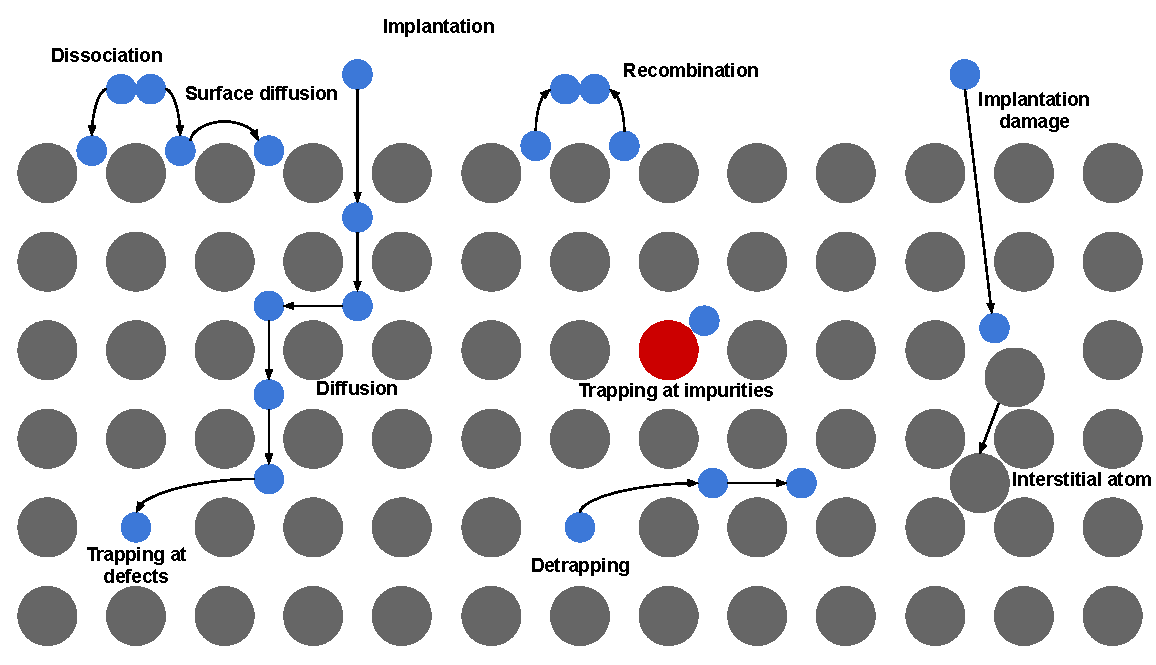
\includegraphics[width=\linewidth]{Figures/Chapter1/HI transport sketch.pdf}
        \caption{Hydrogen.}
    \end{subfigure}
    \begin{subfigure}{0.9\linewidth}
        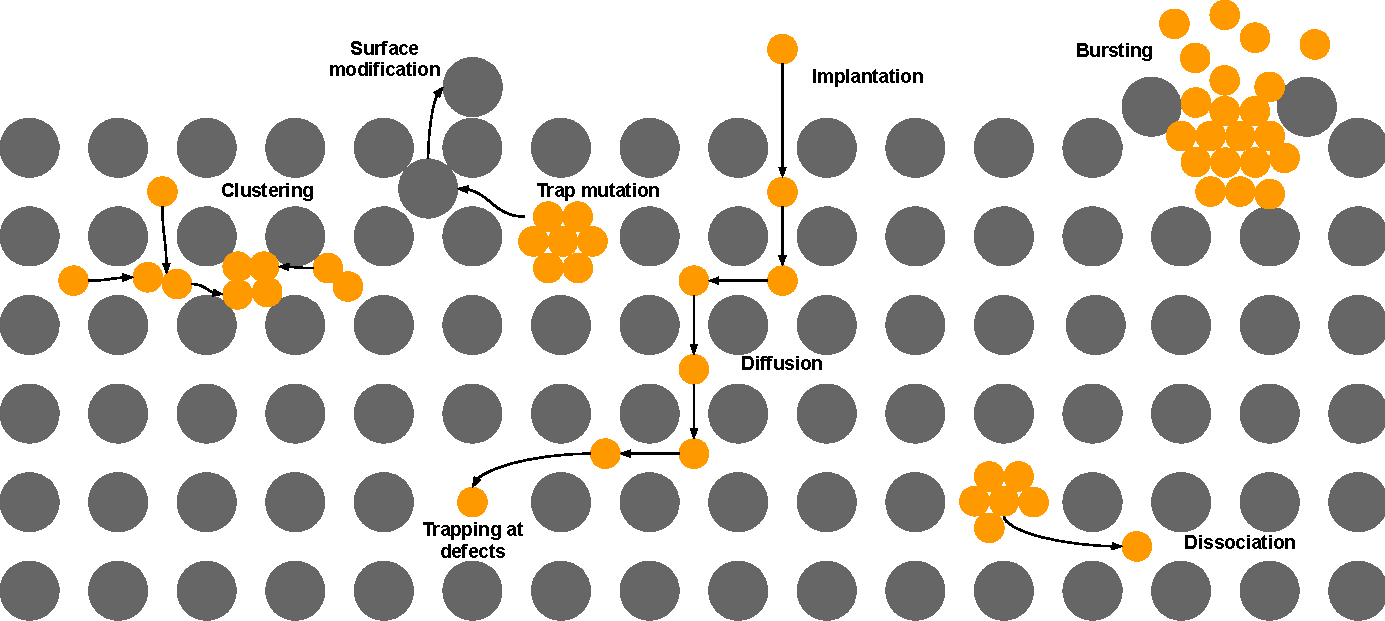
\includegraphics[width=\linewidth]{Figures/Chapter1/He transport sketch.pdf}
        \caption{Helium.}
    \end{subfigure}
    \caption{Interactions of solute species in tungsten.}
    \labfig{helium and hydrogen in metals sketch}
\end{figure*}

\subsection{Particle sources}

\subsubsection{Hydrogen}
Deuterium and tritium being the fuel of fusion reactors, the primary source of hydrogen in the \gls{divertor} is the \gls{plasma} itself.
The wall of a fusion reactor (\gls{first wall} and \gls{divertor}) is bombarded with high energy hydrogen ions.
Due to their small size, these ions can penetrate the metal \gls{lattice} and be implanted in the material.

Components are also exposed to neutral hydrogen particles either in the atomic or molecular form.
This is also the case for the \gls{divertor} region where \gls{fuel recycling} can occur \sidecite{denis_dynamic_2019, causey_hydrogen_2002}.

Tritium can also be produced by the neutron capture of helium-3 \sidecite{shimada_tritium_2017, knoll_radiation_1989} (see \refeq{he3 neutron capture reaction} and \reffig{helium3 neutron capture cross section}).

\begin{equation}
    \ce{^3He + n -> ^1H + ^3H + \SI{0.764}{MeV}}
    \labeq{he3 neutron capture reaction}
\end{equation}

\begin{figure}
    \centering
    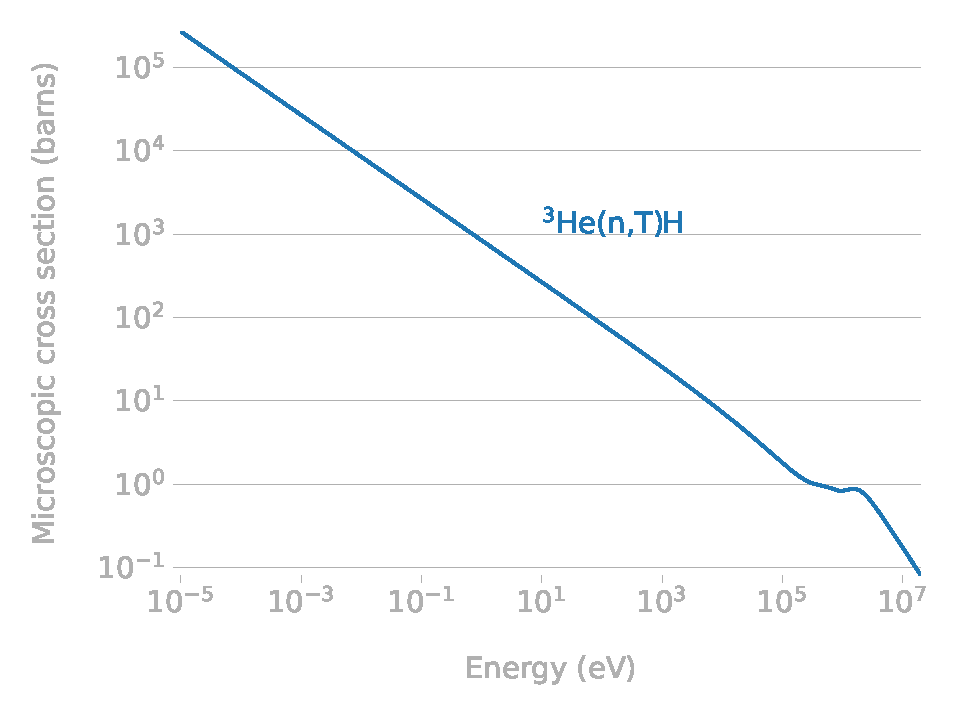
\includegraphics[width=\linewidth]{Figures/Chapter1/cross_section_he3_neutron_capture.pdf}
    \caption{Cross section of the $^3\mathrm{He(n,T)H}$ \cite{shimwell_xsplot_2021}.}
    \labfig{helium3 neutron capture cross section}
\end{figure}

Finally, interactions of lithium with neutrons represent a major source of hydrogen in tritium \glspl{breeding blanket} \sidecite{dark_influence_2021}.

\subsubsection{Helium}\labsec{sources of helium}
Helium is the product of the fusion reaction (see \refeq{fusion reactions}).
Therefore, the wall of a fusion reactor is also bombarded with helium ions.
This is the primary source of helium in \glspl{pfm}.

Helium can also be produced in materials indirectly.
Since tritium decays into helium-3 (see \refeq{tritium decay}), regions with high tritium \gls{retention} are expected to act as a source of helium over time \cite{shimada_tritium_2017}.
Moreover, interactions of neutrons (from the fusion reactions) with metallic elements (e.g.\ tungsten or iron) can produce helium via transmutation \sidecite{watanabe_status_2011}.
This \emph{\gls{transmutation gas}} production has been estimated using well-established neutronics simulations (Monte-Carlo simulations modelling the path of neutroncs in matter) \sidecite{gilbert_neutron-induced_2013, gilbert_integrated_2012}.
Depending on the position in the DEMO \gls{divertor}, cumulative helium production over the course of three \glspl{fpy} could reach more than \SI{400}{appm}.


\subsection{H/W \& He/W interactions}


\begin{figure} [h]
    \centering
    % \begin{subfigure}{\linewidth}
    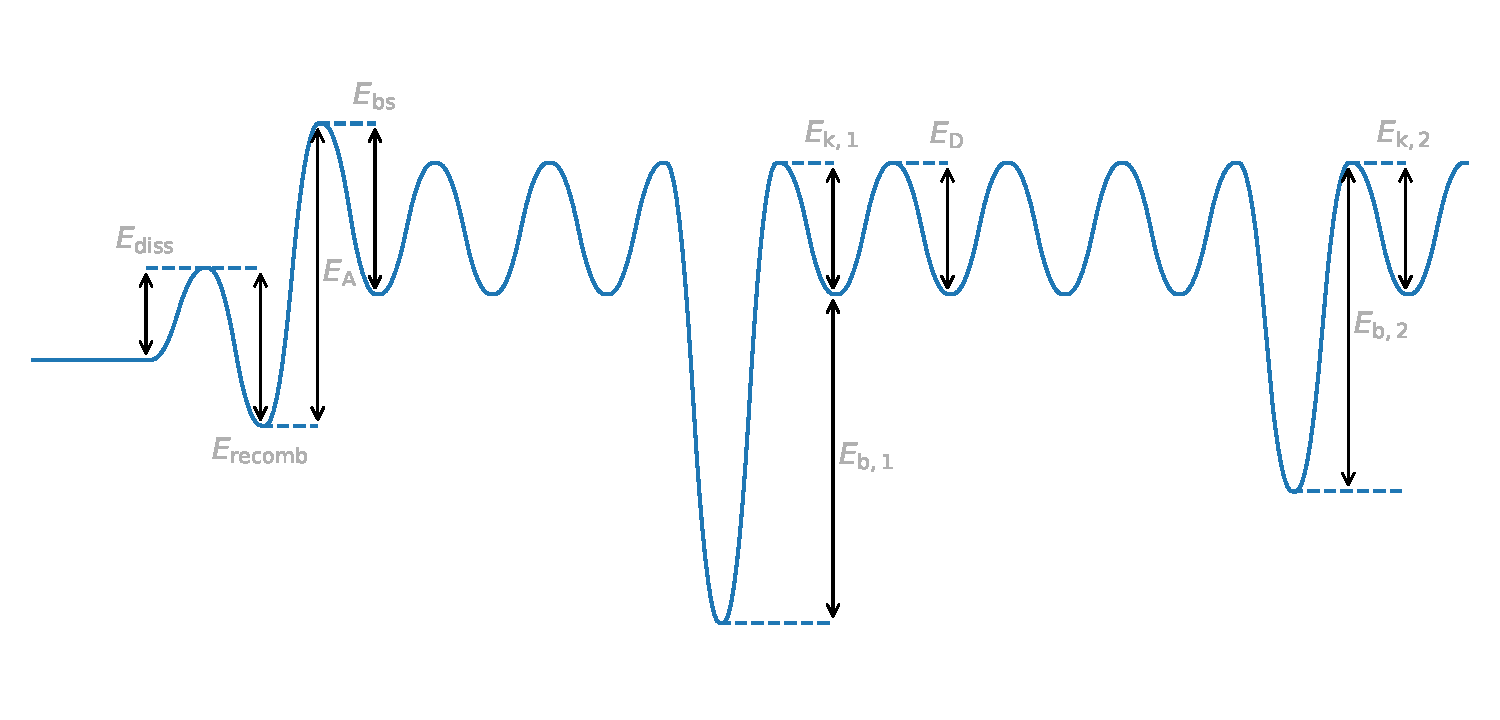
\includegraphics[width=\linewidth]{Figures/Chapter1/potential_energy_diagram.pdf}
    \caption{Simplified potential energy diagram showing two different types of defects.}
    % \end{subfigure}
    % \begin{subfigure}{\linewidth}
    %     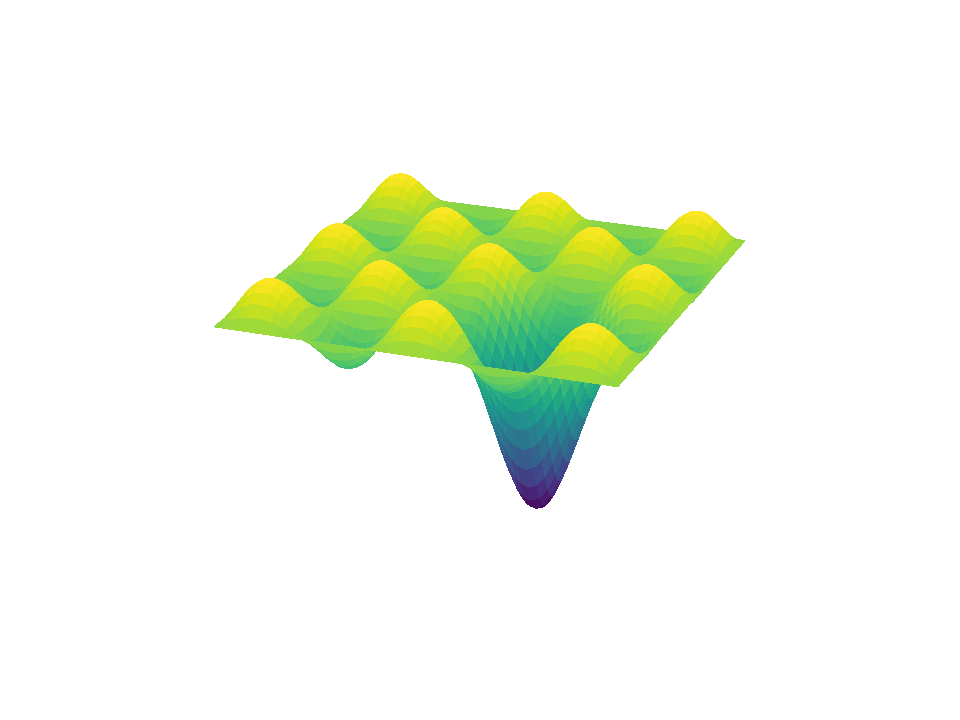
\includegraphics[width=\linewidth]{Figures/Chapter1/potential_energy_3D.pdf}
    %     \caption{3D representation of the potential energy of a solute species in a metal lattice with one defect.}
    % \end{subfigure}
    \labfig{potential energy diagram metal lattice}
\end{figure}

\subsubsection{Diffusion}
The repulsion of metal atoms with solute species creates wells of potential energy located at interstitial sites (see \reffig{potential energy diagram metal lattice}).
The solute atoms in metals can then jump from interstitial site to another thanks to thermal vibration.
This process is called \emph{\gls{diffusion}}.
The `height` of the potential energy wells is called the \gls{diffusion} \textit{activation energy} or \textit{energy barrier} $E_D$.
\Gls{diffusion} is therefore a thermally activated process governed by a diffusion coefficient $D$ expressed in \si{m^2.s^{-1}}, which follows an Arrhenius law:
\begin{equation}
    D = D_0 \exp{(-E_D/k_B T)}
\end{equation}
where $E_D$ is expressed in \si{eV}, $T$ is the temperature in \si{K}, $k_B$ is the Boltzmann constant in \si{eV.K^{-1}}.

\Gls{diffusion} can also be assisted by temperature gradients (called the \emph{\gls{Soret effect}} or \emph{\gls{thermophoresis}}) \sidecite{martinez_thermal_2021, hodille_estimation_2017, longhurst_soret_1985} or hydrostatic pressure gradients.
The tungsten property to simulate the \gls{Soret effect} (Soret coefficient or heat of transport) is currently missing from literature (for hydrogen).
Hodille et al.\ used the properties of steel as an approximation \cite{hodille_estimation_2017}.
Bennanoune and coworkers performed hydrogen transport studies with hydrostatic pressure gradients showing it could have an impact of around \SI{10}{\%} in steel components \sidecite{benannoune_multidimensional_2020}.
% Studies are currently being performed for tungsten.

% MD simulations
Diffusion coefficients (also called diffusivities) can be computed by \gls{md} and \gls{dft}.
The principle of \gls{md} is to calculate the trajectory of atoms in a simulation box (see \reffig{md faney}).
The trajectory of a particle $i$ in a system of $N$ particles can be computed from Newton's second law of motion:

\begin{equation}
    m_i \vec{a_i} = \sum_{j=1 \, j \neq i}^N \vec{F}_{i,j}
\end{equation}
where $m_i$ is the mass of the particle, $\vec{a_i}$ is its acceleration, $\vec{F}_{i,j}$ is the force applied to the particle due to its interaction with particle $j$.
The forces between atoms is only a function of the interatomic potentials.
These potentials can be found in literature or can be estimated from \textit{ab initio} computations (\gls{dft}) \sidecite{boisse_modelling_2014,boisse_modeling_2014} or from methods based on machine learning \sidecite{lam_modeling_2021,behler_constructing_2015}.

\begin{figure*}
    \centering
    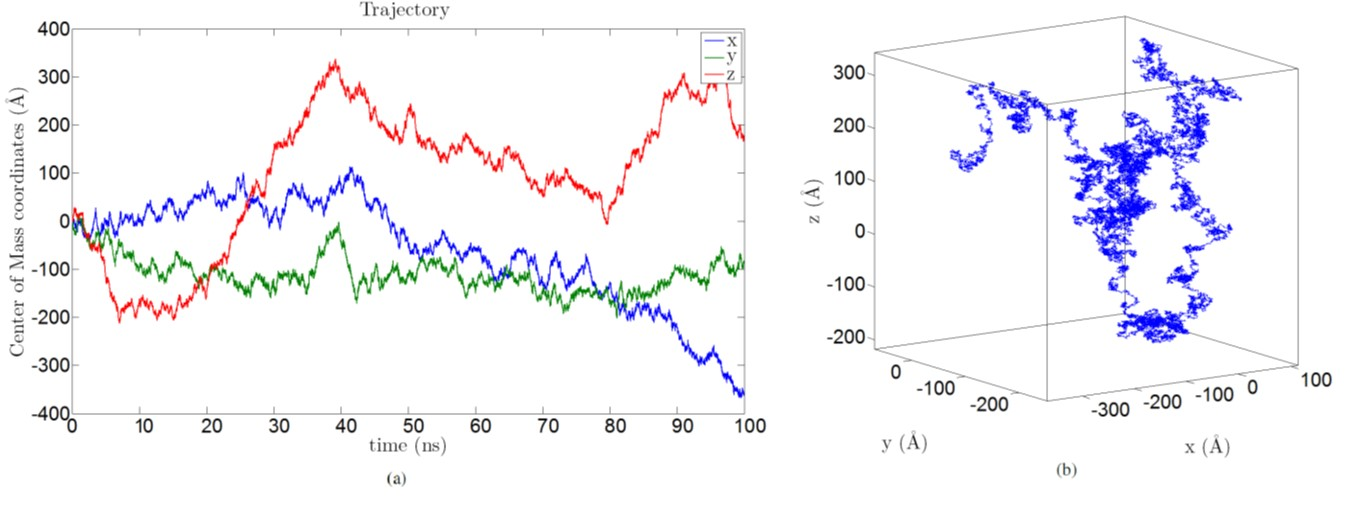
\includegraphics[width=\linewidth]{Figures/Chapter1/faney_md.jpg}
    \caption{Example of the trajectory of a He$_2$ cluster in tungsten. Reproduced from \cite{faney_numerical_2013}.}
    \labfig{md faney}
\end{figure*}

By measuring the trajectory of a diffusing species from \gls{md} simulations for a long time, its diffusion coefficient $D$ can be estimated from Einstein equation \cite{einstein_uber_1905}:
\begin{equation}
    \lim_{t\to\infty} \frac{\langle R^2(t) \rangle}{6t} = D
\end{equation}
where $\langle R^2(t) \rangle$ is the mean squared displacement of the species.

This modelling technique was used to estimate the diffusion coefficient of \gls{H} in \gls{W} \sidecite{wang_molecular_2020, zhou_molecular_2016,kato_super-saturated_2015,liu_hydrogen_2014} and for He in \gls{W} \sidecite{faney_numerical_2013,faney_spatially_2014,faney_spatially_2015,sefta_surface_2013,perez_mobility_2017}.

% Experiments
Diffusivity of hydrogen has also been measured experimentally in \gls{W} \sidecite{holzner_solute_2020, frauenfelder_solution_1969, anderl_hydrogen_1990}, copper and copper alloys (CuCrZr) \sidecite{anderl_deuterium_1992} and other metals.
Note that the diffusion coefficients measured experimentally are usually effective coefficients accounting for \gls{trapping} effects (detailed below).
% EUROFER \sidecite{montupet-leblond_permeation_2021,esteban_hydrogen_2007,aiello_hydrogen_2002}, 
Because He tends to cluster (as explained below), measuring its diffusivity experimentally is extremely complicated and therefore most estimations of He diffusion coefficients are numerical.
\reffig{diffusivity materials} is a collection of diffusivity values found in literature (measured experimentally or computed) for tungsten, copper and CuCrZr.

% The diffusivities of copper and CuCrZr are comparable (see \reffig{diffusivity solubility copper} and \reffig{diffusivity solubility cucrzr}).

\begin{figure}
    \centering
    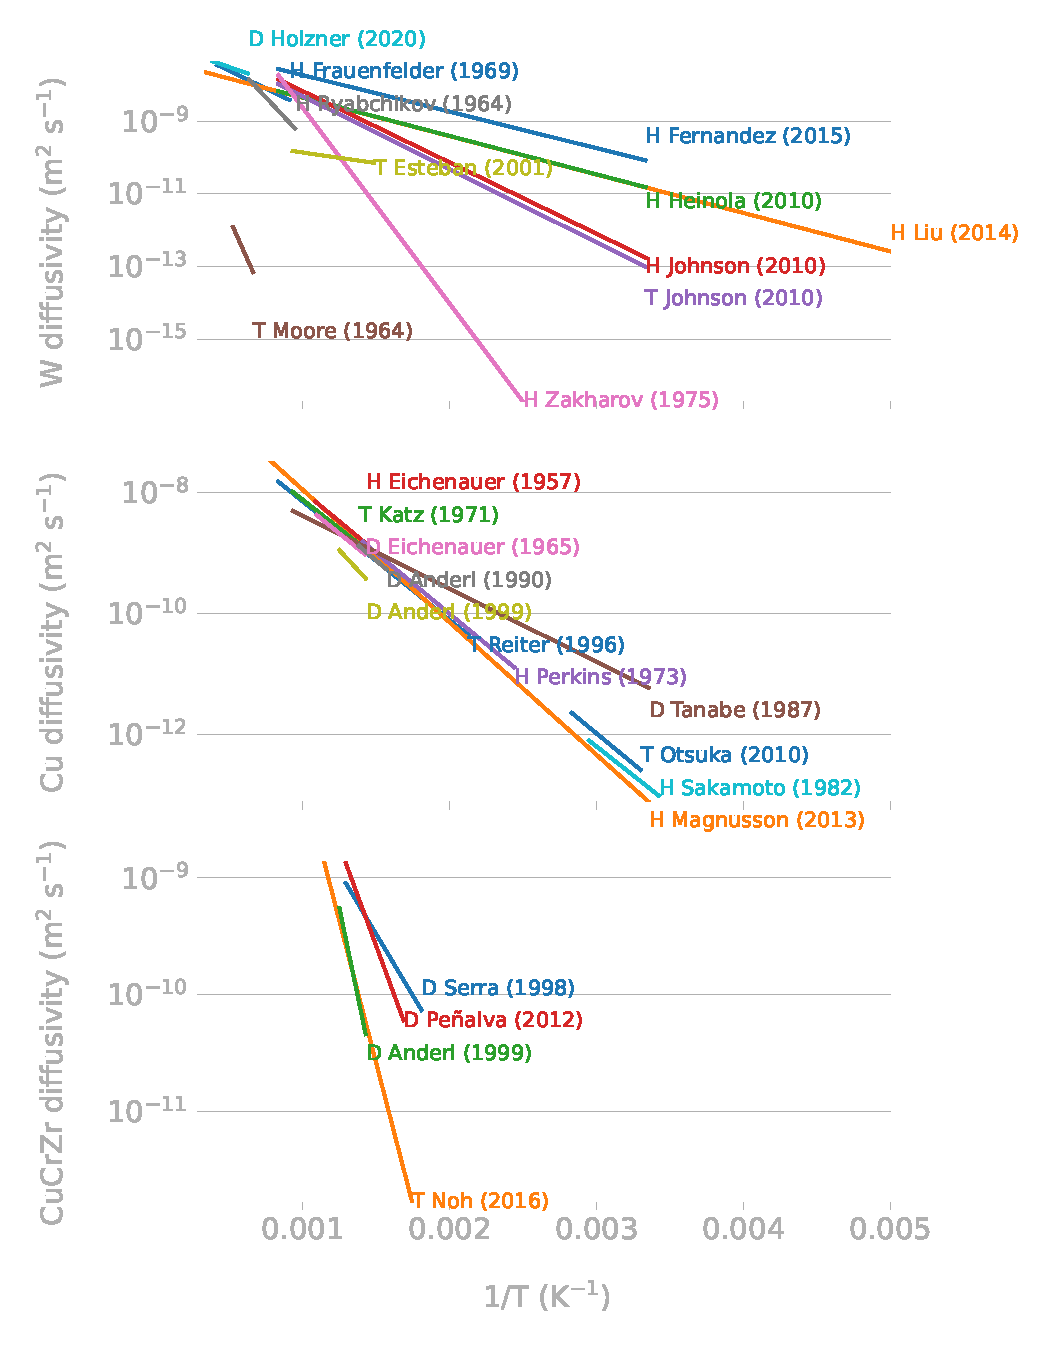
\includegraphics[width=0.8\linewidth]{Figures/Chapter1/materials_diffusivity_review_comparison.pdf}
    \caption{Diffusivity values for tungsten, copper and CuCrZr. Data from \cite{delaporte-mathurin_remdelaportemathurinh-transport-materials_2022}.}
    \labfig{diffusivity materials}
\end{figure}

\subsubsection{Trapping at defects}

Due to the repulsion between solute species and the surrounding metal atoms, defects can act as wells of potential energy for solute species (see \reffig{potential energy diagram metal lattice}).
Once in that attractive well, species can escape it only if their kinetic energy (i.e.\ the temperature) is high enough.
Species can be trapped at \glspl{vacancy}, \glspl{dislocation loop}, \gls{self-interstitial} atoms (in the case of hydrogen in tungsten), impurities, etc.

The \gls{trapping} process can be described as:
\begin{equation}
    \ce{H + [\quad] <=>[k][p] [H]}
\end{equation}
where H is the particle in an interstitial site (i.e.\ mobile), $[\quad]$ is the defect and $[\mathrm{H}]$ represents the particle trapped in the defect.
The \gls{trapping} rate and \gls{detrapping} rate can be respectively expressed as:
\begin{align}
    k &= k_0 \exp{\frac{-E_k}{k_B T}} \\
    p &= p_0 \exp{\frac{-(E_\mathrm{b} + E_k)}{k_B T}} = p_0 \exp{\frac{-E_p}{k_B T}}
\end{align}
where $E_k$ is the \gls{trapping} energy in \si{eV}, $k_B$ is the Boltzmann constant in \si{eV.K^{-1}}, $T$ is the temperature in \si{K}, $E_\mathrm{b}$ is the binding energy of the particle with the defect and $E_p = E_\mathrm{b} + E_k$ is the \gls{detrapping} energy.
A common assumption is that $E_k = E_D$.

Each rate therefore has two parameters: the pre-activation factor and the activation energy.
These parameters can be identified from fitting \gls{tds} experiments.
\gls{tds} experiments consist in loading a metal sample with the studied species (e.g.\ \gls{H} or \gls{He}) and heat it at different temperatures with a well controlled temperature ramp (e.g.\ \SI{1}{K.s^{-1}}, \SI{10}{K.s^{-1}}...) while measuring the desorption flux.
This results in a spectrum which typically has one or several desorption peaks corresponding to different traps (see \reffig{TDS example ialovega}).
Peaks appearing at high temperatures correspond to ``deep'' traps with a high \gls{detrapping} energy $E_p$.

\begin{figure*}
    \centering
    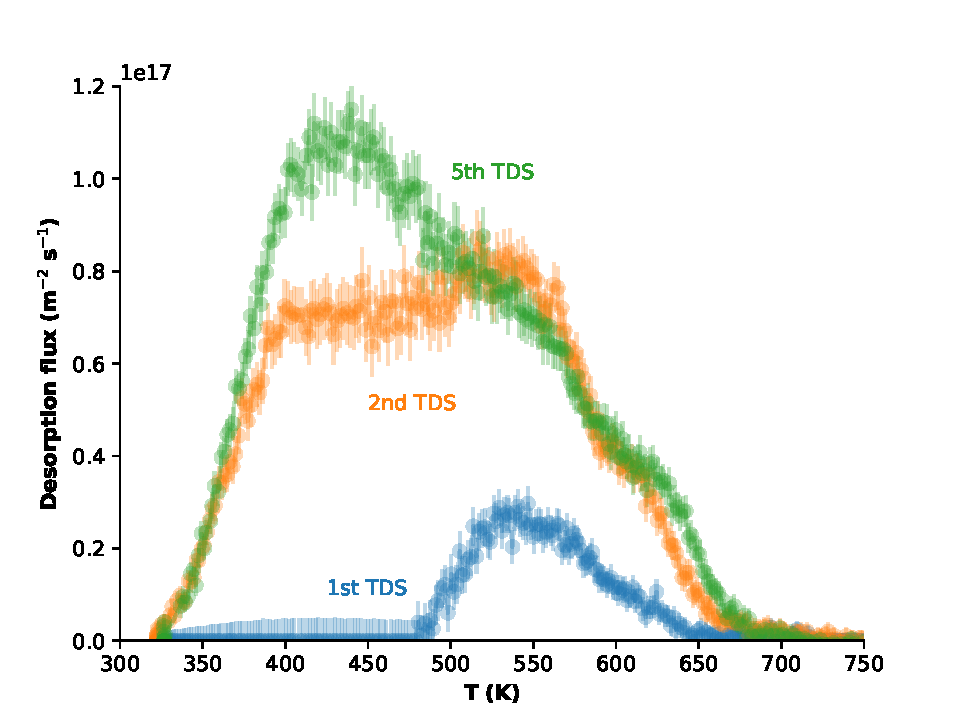
\includegraphics[width=0.75\linewidth]{Figures/Chapter1/tds_helium_nicolas.pdf}
    \caption{H TDS spectra of pre-damaged W. Reproduced from \cite{ialovega_hydrogen_2020}.}
    \labfig{TDS example ialovega}
\end{figure*}

These parameters can also be obtained from \gls{dft} calculations \sidecite{hou_predictive_2019, backer_hydrogen_2017, backer_multiscale_2017, fernandez_hydrogen_2015, lu_review_2014, heinola_hydrogen_2010, zhou_investigating_2010}.

Some defects can trap several hydrogen/helium atoms.
For instance, up to approximately seven helium atoms can be trapped in a mono-\gls{vacancy} at room temperature \sidecite{faney_spatially_2015}.
\gls{dft} calculations also show that defects like mono-vacancies, dislocations or grain boundaries can retain multiple hydrogen atoms (see \reffig{trapping energy hydrogen in tungsten}).
As the number of trapped particles (helium or hydrogen) increases, the binding energy of a particle with the defect usually decreases.
In other words, the more particles are trapped in a defect the easier it is for a hydrogen atom to escape.
For instance, the binding energy of a helium atom in an empty mono-\gls{vacancy} is around \SI{4}{eV} and around \SI{2.5}{eV} if the \gls{vacancy} already retains four helium atoms \cite{faney_spatially_2015}.
Similarly, the binding energy of a hydrogen atom in a mono-\gls{vacancy} varies from \SI{0.5}{eV} (with six hydrogen atoms trapped) to \SI{1.3}{eV} (empty \gls{vacancy}) (see \reffig{trapping energy hydrogen in tungsten}).

\begin{figure*}
    \centering
    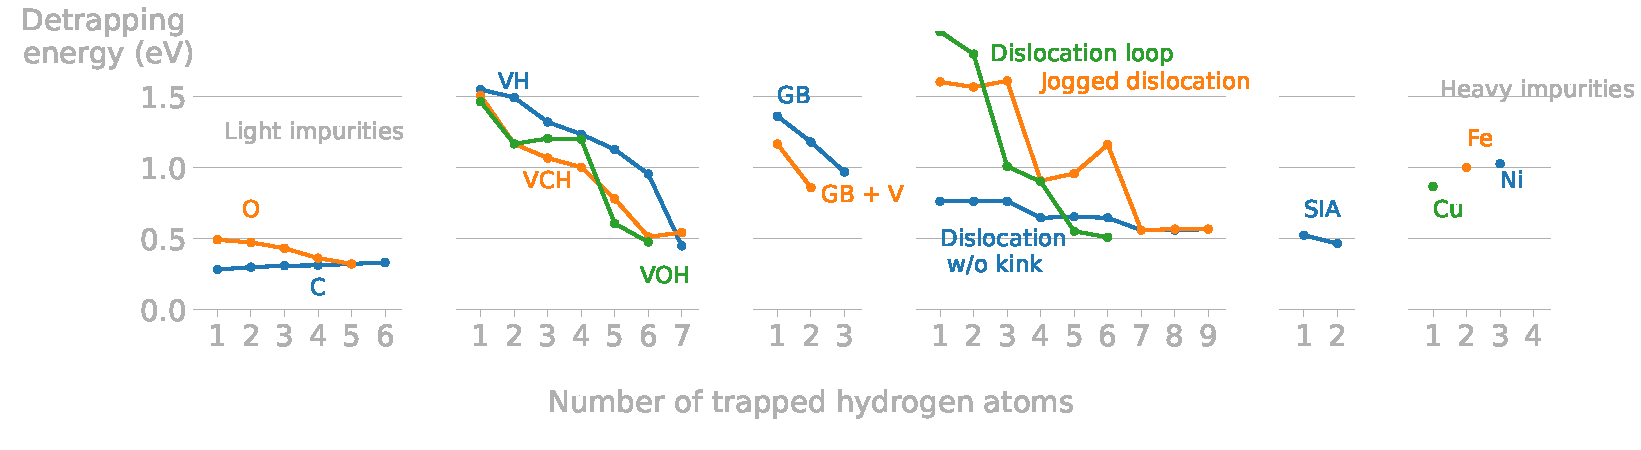
\includegraphics[width=\linewidth]{Figures/Chapter1/trapping_energy_hydrogen_in_tungsten.pdf}
    \caption{Detrapping energy of a hydrogen atom in several defects in tungsten: vacancies, impurities, self-interstitial atoms (SIA), grain boundaries (GB), in tungsten depending on the number of trapped hydrogen atoms. Reproduced from \cite{hodille_study_2016}.}
    \labfig{trapping energy hydrogen in tungsten}
\end{figure*}

Defects can either be pre-existent in the material (sometimes called \textit{intrinsic} defects): impurities, grain boundaries, etc.
They can also be created from external factors (\textit{extrinsic} defects) like particle bombardment (ions, neutrons) \sidecite{ogorodnikova_deuterium_2003} or mechanical stress \sidecite{benannoune_multidimensional_2020}.

\subsubsection{Surface dissolution}

When a surface is in contact with a gas, molecular species (e.g.\ $\text{H}_2$, $\text{T}_2$, $\text{HD}$...) can dissociate into mono-atomic species.
After their dissociation, the atomic particles can be adsorbed on the surface (on adsorption sites).
This dissociation is described by a sticking probability usually associated with an Arrhenius law $s = s_0 \exp{(-E_s/k_B T)}$.
\gls{dft} calculations can calculate energy barriers for adsorption and migration of solute species on surfaces \sidecite{heinola_first-principles_2010}.
Studies have however shown that this process is not thermally activated (i.e.\ $E_s=0$) \sidecite{alnot_adsorption_1989, tamm_interaction_1970} but rather depends on the ratio of the surface concentration of the species (hydrogen or helium) by the concentration of adsorption sites.
This quantity is called the \textit{surface coverage} $\theta$. 
When $\theta = 1$, the surface is fully saturated and when $\theta = 0$ all the adsorption sites are available.
Moreover, the presence of impurities occupying adsorption sites can decrease the sticking probability of a species \sidecite{dunand_surface_2022, whitten_coadsorption_1998}.

Adsorbed particles can then be \textit{absorbed} in the bulk (see \reffig{potential energy diagram metal lattice}).
This thermally activated process is associated with an absorption coefficient following an Arrhenius law $A=A_0 \exp{(-E_A/k_B T)}$.
The absorption process is modelled using \gls{dft} and absorption activation energies $E_A$ can be determined for different surface orientations \sidecite{johnson_hydrogen_2010, nojima_theoretical_2007,ajmalghan_surface_2019}.

All these processes (dissociation, adsorption and absorption) can be described by an absorption flux:
\begin{equation}
    \varphi_\mathrm{abs} = n K_\mathrm{abs} P
\end{equation}
where $n$ is the absorption order, $K_\mathrm{abs}$ is the absorption coefficient expressed in \si{m^{-2}.s^{-1}.Pa^{-1}} and $P$ is the partial pressure of hydrogen in \si{Pa}.

Desorption of solute species at the surface is expressed by a desorption flux:
\begin{equation}
    \varphi_\mathrm{des} = K_\mathrm{des} c_\mathrm{surface}^n
\end{equation}
where $K_\mathrm{des}$ is the desorption coefficient expressed in \si{m^{-2+3n}.s^{-1}}, $c_\mathrm{surface}$ is the surface concentration in \si{m^{-3}}, and $n$ is the order of the desorption.

When the equilibrium between absorption and desorption is reached, $\varphi_\mathrm{abs} = \varphi_\mathrm{des}$, which gives:
\begin{equation}
    n K_\mathrm{abs} P = K_\mathrm{des} c_\mathrm{surface}^n
    \labeq{equilibrium absorption desorption}
\end{equation}

By rearranging \refeq{equilibrium absorption desorption}:
\begin{equation}
    c_\mathrm{surface} = \sqrt[n]{n \frac{K_\mathrm{abs}}{K_\mathrm{des}}} \sqrt[n]{P}
\end{equation}

When the absorption/desorption order is $n=1$ (monoatomic absorption):
\begin{equation}
    c_\mathrm{surface} = S P
\end{equation}
This relationship is known as Henry's law of solubility and $S = K_\mathrm{abs}/K_\mathrm{des}$ is the material solubility expressed in \si{m^{-3}.Pa^{-1}}.

When the absorption/desorption order is $n=2$ (diatomic absorption):
\begin{equation}
    c_\mathrm{surface} = S \sqrt{P}
    \labeq{sievert's law}
\end{equation}
This equiilbrium is known as Sievert's law of solubility and $S = \sqrt{2 K_\mathrm{abs}/K_\mathrm{des}}$ is the material solubility expressed in \si{m^{-3}.Pa^{-0.5}}.
The solubility of tungsten, copper and CuCrZr are described in \reffig{solubility materials}.

The product of the solubility and diffusivity is called \textit{permeability}.

\begin{figure}
    \centering
    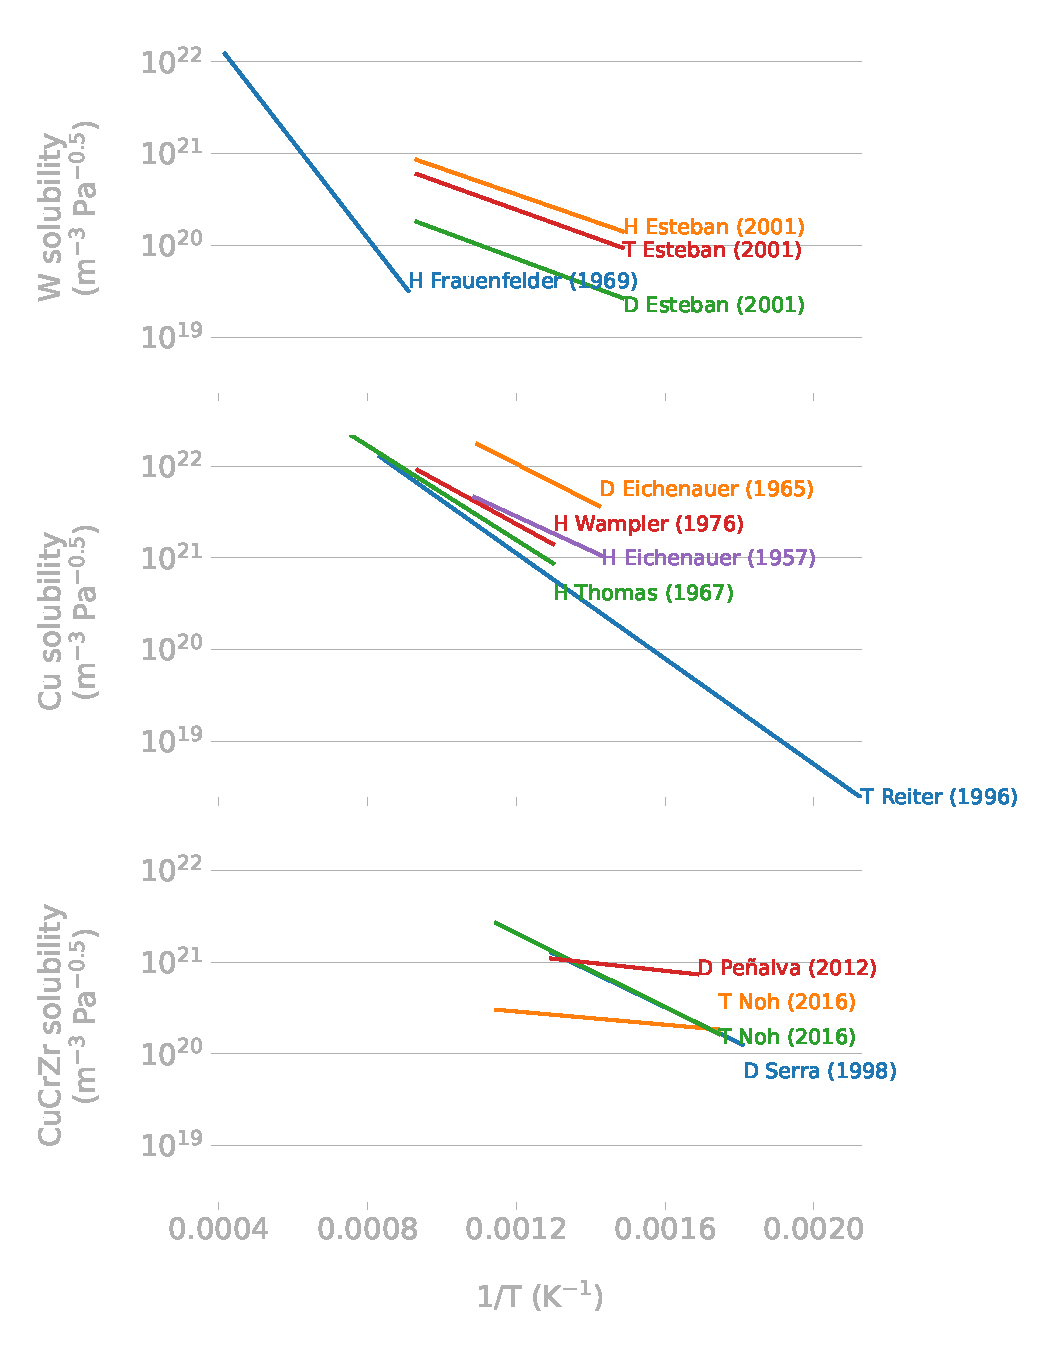
\includegraphics[width=0.75\linewidth]{Figures/Chapter1/materials_solubility_review_comparison.pdf}
    \caption{Solubitity values for tungsten, copper and CuCrZr. Data from \cite{delaporte-mathurin_remdelaportemathurinh-transport-materials_2022}.}
    \labfig{solubility materials}
\end{figure}

\subsubsection{Interface between materials}
At the interface between two materials, the continuity of chemical potential has to be ensured \sidecite{krom_hydrogen_2000}.
The continuity of chemical potential is conveyed by the continuity of $P$, the local partial pressure of hydrogen at equilibrium.
In a metal, $P$ can be expressed from Sievert's law of solubility (see \refeq{sievert's law}):
\begin{equation}
    P = (c_\mathrm{m}^-/S^-)^2
\end{equation}
with $c_\mathrm{m}$ the concentration of mobile species in the material, $S$ the solubility in the materials expressed in \si{m^{-3}.Pa^{-0.5}}.
% A way to picture the continuity of chemical potential is to imagine a gas layer at the interface between two materials at a partial pressure $P_\mathrm{eq}$.
% $P_\mathrm{eq}$ can be expressed by the solubility law at the surface of each material.
At the interface between two metallic surfaces, the chemical potential continuity is therefore conveyed by the continuity of the quantity $c_\mathrm{m}/S$:
\begin{equation}
    (c_\mathrm{m}^-/S^-)^2 = (c_\mathrm{m}^+/S^+)^2
    \labeq{c/s conservation}
\end{equation}

In the case of a metal in contact with a non-metallic liquid behaving according to Henry's law (e.g.\ a molten salt):
\begin{equation}
    (c_\mathrm{m}^-/S^-)^2 = c_\mathrm{m}^+/S^+
\end{equation}
with $S$ the solubility of \gls{H} in the materials expressed in \si{m^{-3}.Pa^{-0.5}} or \si{m^{-3}.Pa^{-1}}.

A jump in concentration will therefore occur at the interface between two materials with different solubilities.

\subsubsection{Advection in liquids}
\Gls{advection} occurs when a mobile species is in a liquid (molten salts, water, coolants...) and depends on the liquid velocity.
This advective transport adds up to the diffusive transport.

Depending on the liquid velocity and the species diffusivity in this liquid, the mass transport can be predominated by one of the two phenomena.
The Péclet number $\mathrm{Pe}$ is a dimensionless number employed to estimate this dominance.

\begin{equation}
    \mathrm{Pe} = \frac{\mathrm{advective \; transport \; rate}}{\mathrm{diffusive \; transport \; rate}} = \frac{L u}{D}
\end{equation}
where $L$ is a characteristic length, $u$ is the fluid velocity and $D$ is the species diffusivity in this fluid.

When $\mathrm{Pe} \gg 1$, \gls{advection} is the dominant transport phenomena.
When $\mathrm{Pe} \ll 1$, \gls{diffusion} dominates and \gls{advection} can be neglected.

For hydrogen diffusing in liquid LiPb (typically in a WCLL breeding blanket with a characteristic length $L \approx \SI{1}{m}$), with $D \approx \SI{1e-9}{m^2.s^{-1}}$ and $u \approx \SI{1e-4}{m.s^{-1}}$ \sidecite{dark_influence_2021}, $\mathrm{Pe} \approx 10^{5}$, which means that \gls{advection} dominates the mass transport and cannot be neglected.

\subsubsection{Clustering}
Single He atoms implanted into the material diffuse rapidly due to the high W-He repulsion.
This high repulsive W-He interaction is such that interstitial He atoms preferably rearrange into groups of atoms in order to minimise the number of repulsive interactions \sidecite{hamid_molecular_2019, hammond_large-scale_2018}.
This phenomenon, called \emph{clustering}, was highlighted by \gls{dft} studies \cite{becquart_density_2009,dunn_rate_2013} and MD simulations \cite{henriksson_molecular_2006}.
Small clusters are themselves mobile as long as all the He atoms within the cluster are occupying interstitial position in the solid \gls{lattice}.
The activation energy for interstitial He atoms and clusters in \gls{W} ranges from 0.15 to \SI{0.45}{eV} according to Perez et al.\ \sidecite{perez_mobility_2017}.
He clusters will eventually grow by interacting with either interstitial He atoms or other clusters.

Clustering of \gls{H} atoms is less clear and Henriksson et al.\ showed that \gls{H} atoms do not form bonds with other \gls{H} atoms in \gls{bcc} \gls{W} \sidecite{henriksson_difference_2005}.

\subsubsection{Bubble nucleation}

If its size is big enough the cluster pressure is sufficient to knock off a \gls{W} atom from the \gls{lattice}, creating a \gls{W} \gls{vacancy} and an interstitial \gls{W} atom (a \gls{Frenkel pair}).
This process is called \gls{trap mutation} or \emph{\gls{self-trapping}} and the trapped clusters act as nuclei for bubble formation.

\Gls{trap mutation} has been modelled in \gls{W} using \gls{dft} \sidecite{boisse_modelling_2014} and Monte Carlo computations \sidecite{de_backer_modeling_2015}.
It has been shown that this phenomenon depends not only on the number of He atoms in the cluster but also on temperature, position of the cluster to the free surface or even the crystal orientation \sidecite{blondel_modeling_2017, hu_interactions_2014, hu_dynamics_2014}.
At this point, the trapped cluster occupies the newly created \gls{W} \gls{vacancy} position.
It is considered immobile since it would require either diffusion of another \gls{vacancy} next to it, or recombination of the Frenkel pair in order to diffuse \sidecite{morishita_nucleation_2007}.

\subsubsection{Bubble growth}

\begin{figure} [h!]
    \centering
    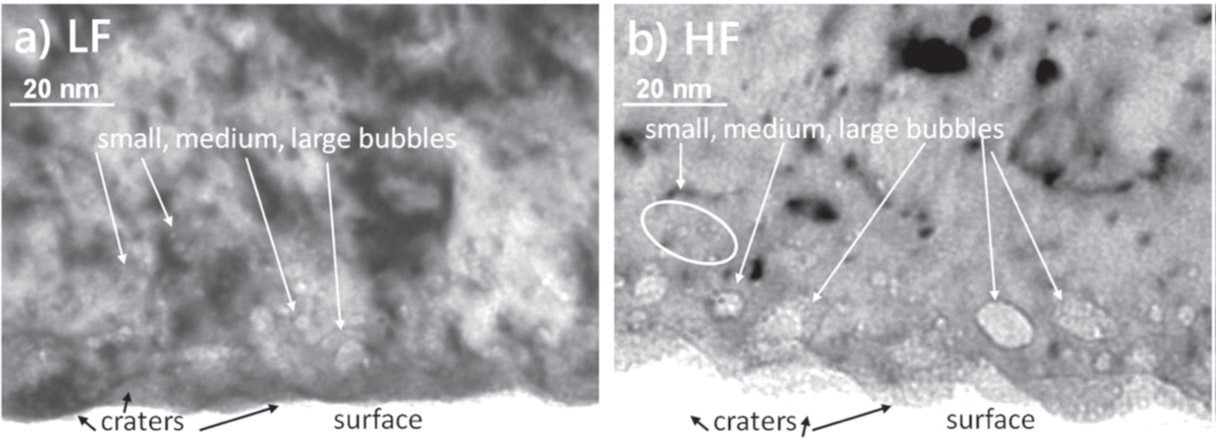
\includegraphics[width=\linewidth]{Figures/Chapter1/helium_bubbles_ialovega.jpg}
    \caption{Transmission electron microscopy image of tungsten irradiated with He ions at different fluxes (Low Flux (LF) = \SI{2.9e20}{m^{-2}.s^{-1}} and High Flux (HF) = \SI{2.3e22}{m^{-2}.s^{-1}}) showing the presence of He bubbles. Reproduced from \cite{ialovega_hydrogen_2020}.}
    \labfig{he bubbles ialovega}
\end{figure}

Once a bubble nucleus is created via \gls{trap mutation}, it can continue to grow by absorbing other clusters.
Two or more bubbles can also coalesce and form a bigger bubble.
Condon and Schober \sidecite{condon_hydrogen_1993} reviewed the key mechanisms of bubble growth in metals.

Each of these mechanisms can become dominant over another depending on the implantation and the metal conditions. 
Bubbles can continue to grow by absorbing interstitial He atoms or mobile He clusters (i.e.\ that haven't self trapped).
Considering that vacancies are mobile in the solid, the volume of a bubble could also increase if a \gls{vacancy} or a \gls{vacancy} cluster interacts with a He bubble.
The same is true for He-vacancies or H-vacancies clusters.

There is no experimental evidence of He clustering with \gls{self-interstitial} \gls{W} atoms \sidecite{faney_spatially_2014}.

% This process is described by cluster dynamics equations in which interaction between the clusters is governed by pairs of association and dissociation rates.
During the growth of a He bubble by absorbing He atoms, if the pressure increases until reaching a critical value, \gls{dislocation loop} punching can occur.
During the punching event, a whole facet of \gls{W} atoms is pushed, and the vacant \gls{lattice} sites are absorbed by the bubble allowing the bubble to expand and reducing the pressure in it \sidecite{sefta_surface_2013}.
The produced \gls{self-interstitial} \gls{W} atoms will likely be attracted by \textit{image forces} at the surface and will contribute to the roughening of the surface and/or formation of surface structures.

\Glspl{dislocation loop} happen at very high pressure and if the number of vacancies in the \gls{lattice} is low compared to the amount of He atoms.
This is the case when a high He flux is applied and the He ions energy is low so that no displacement damaged is produced \cite{sefta_surface_2013}.
If vacancies were created via He ions implantation, they could interact with existing He bubbles which would have the effect of increasing the volume and thus decreasing the pressure (assuming no change in temperature and no other implantation mechanism).

Coalescence of He bubbles has been observed in \gls{md} simulations \sidecite{hamid_molecular_2019, hammond_helium_2019, zhang_simulation_2019} and would tend to increase the bubble size decreasing the bubble density at the same time.
This may not have an impact on He concentration on the macroscopic scale but might influence bubble bursting.

The pressure inside the bubble and the bubble radius are two parameters of interest and are correlated.
Sefta \sidecite{sefta_surface_2013} proposed to use the Wolfer equation of state in order to determine the number of He atoms contained in a He bubble based on its pressure, the latter being calculated from its radius and its surface tension.
One must be aware that if radii and pressure of bubbles computation is quite straightforward using \gls{md} \sidecite{zhang_simulation_2019} or cluster dynamics \sidecite{faney_spatially_2015} simulations it will be more complex to estimate these metrics considering a continuum model that does not keep track of every type of clusters but only a few of them.
The only information \textit{a priori} available in this case is indeed the local helium concentration and an equivalence could be found by either having a high density of small bubbles or a low density of big bubbles.
An effort has been made by Ialovega to measure the pressure inside helium bubbles using \gls{eels} \sidecite{ialovega_surface_2021}.
This technique, consisting in analysing the electron energy loss as they interact with matter \sidecite{pyper_excited_2017}, showed evidence that the observed cavities (see \reffig{he bubbles ialovega}) were filled with helium.

Ultimately, a bubble can form blisters, increase its size via \gls{loop punching} or even burst.

\subsubsection{Blistering}

\begin{figure}
    \centering
    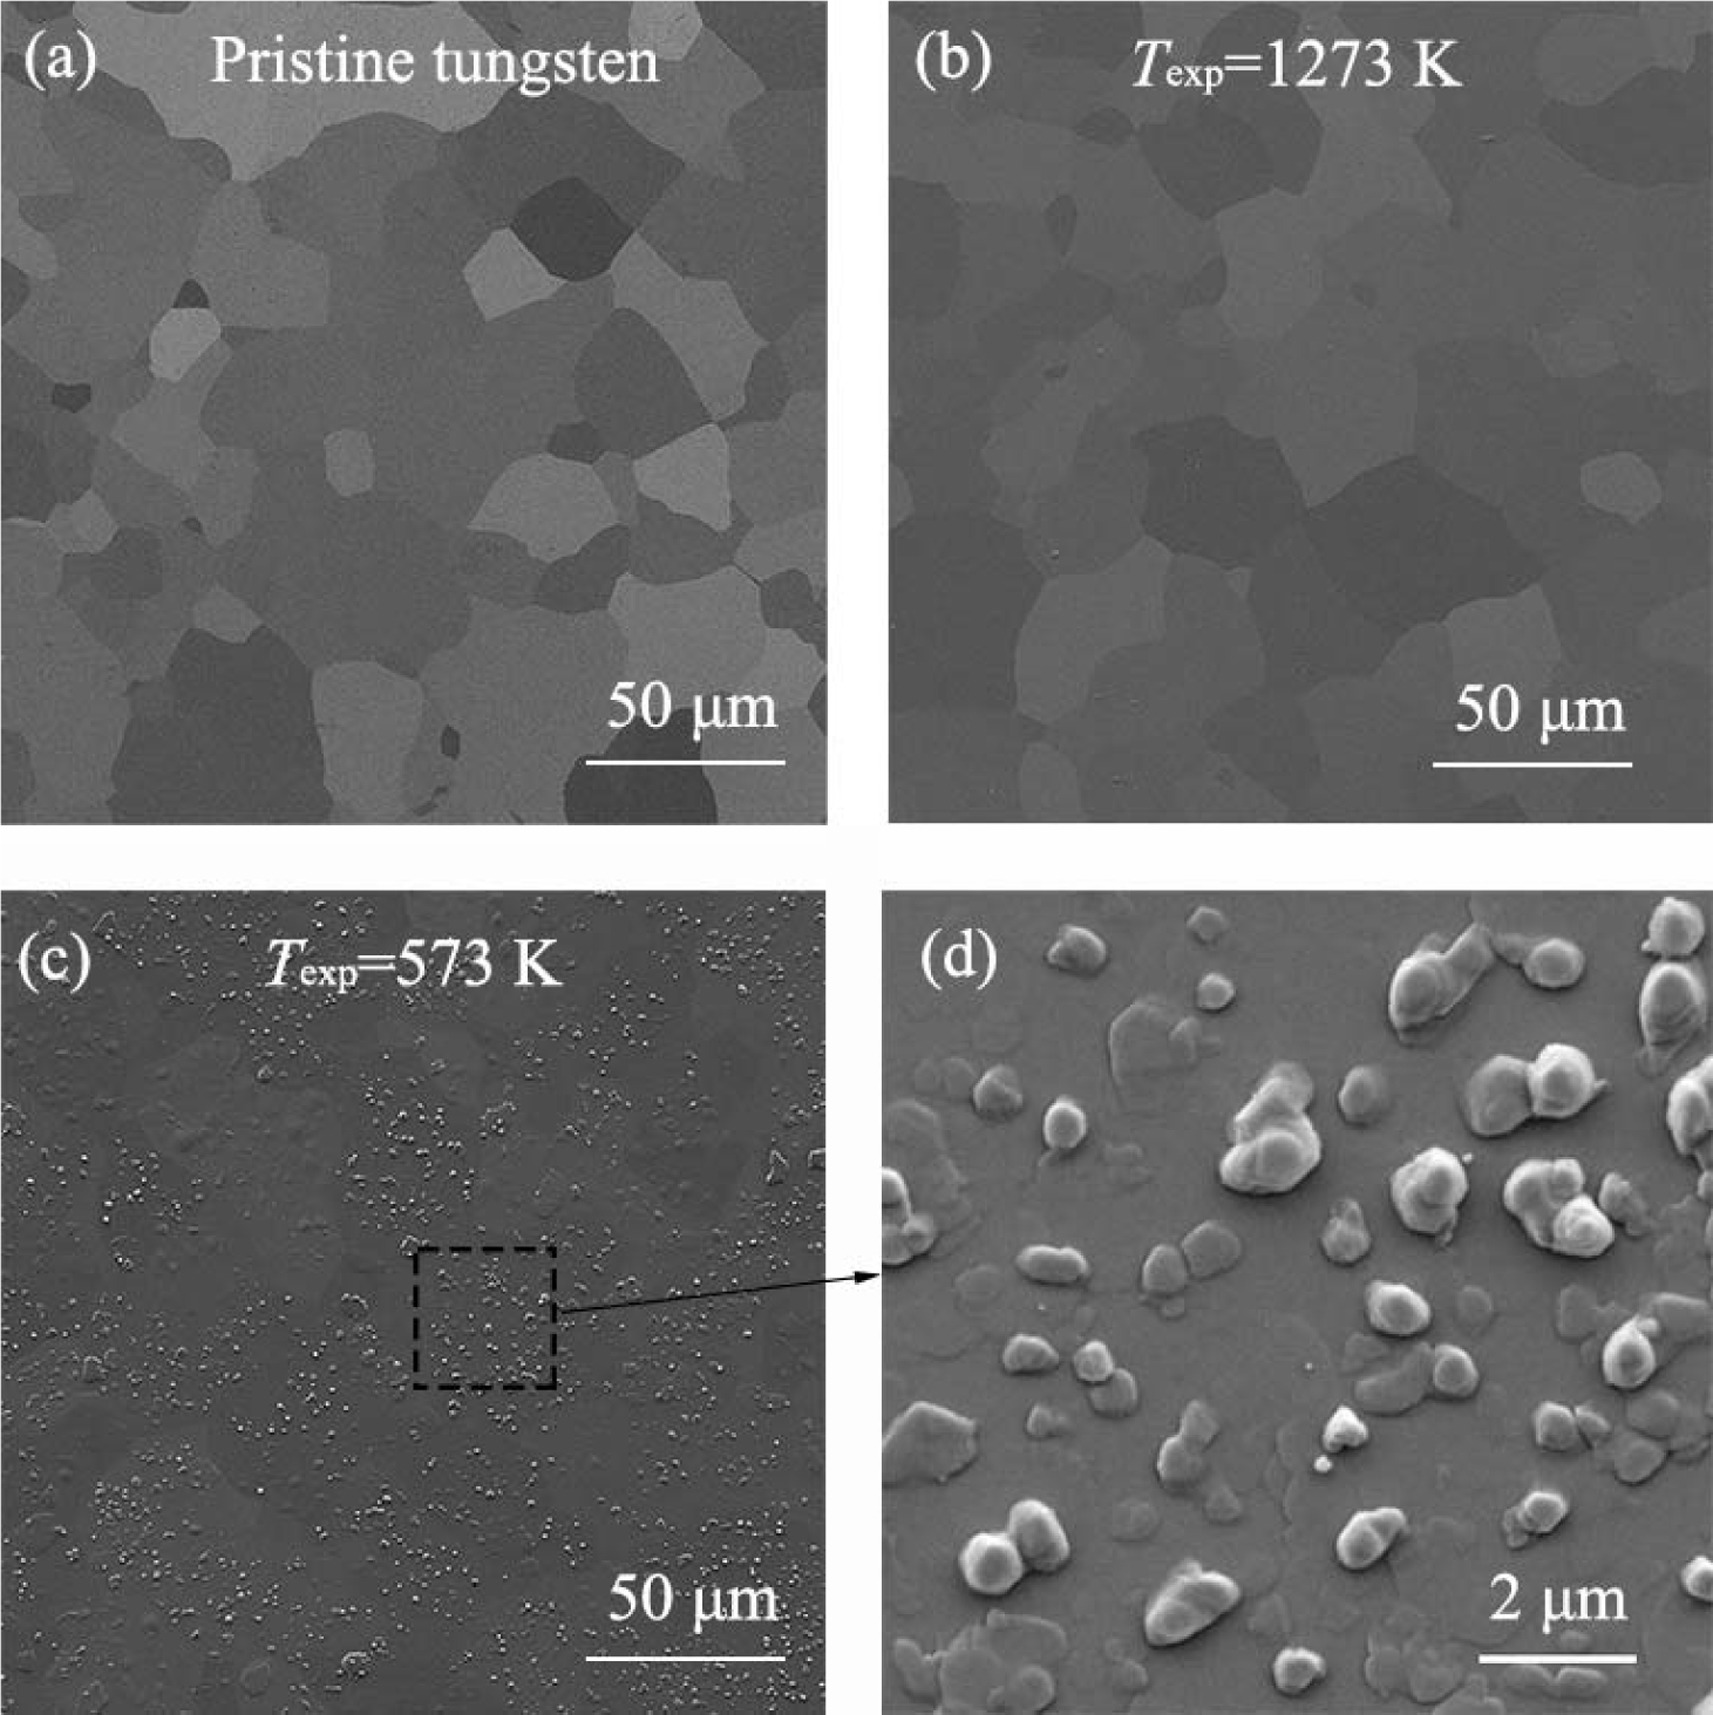
\includegraphics[width=\linewidth]{Figures/Chapter1/h_blisters_in_tungsten.jpg}
    \caption{Scanning Electron Microscopy images of the surface of W samples exposed to \SI{50}{eV} H plasma at \SI{573}{K} and \SI{1273}{K}. Reproduced from \cite{chen_irradiation_2019}.}
    \labfig{h blisters in tungsten}
\end{figure}

During helium or hydrogen implantation, \emph{\gls{blistering}} can be observed under certain conditions.
Blisters are plastic deformation (swelling) of the metal near the surface due to high pressure in bubbles (see \reffig{h blisters in tungsten}).
This phenomenon is separated from \gls{loop punching} even though \gls{loop punching} can be considered as a plastic deformation.
\Gls{blistering} usually happens at low temperatures because only then the growth rate of the bubble is greater than the dissolution in the bulk (which depends on the thermally activated diffusion coefficient and solubility).
Eventually, if the rate of incoming atoms is greater that the rate of re-dissolution in the bulk, blisters can rupture.
Similarly, if the rate of incoming atoms is less than the rate of re-dissolution in the bulk, the blister will collapse.

Helium \gls{blistering} has been observed in \gls{W} at low temperature ($< \SI{1000}{K}$) \sidecite{baldwin_formation_2010}.
Hydrogen \gls{blistering} was also observed in \gls{W} \sidecite{haasz_effect_1999}.
Causey et al.\ also reviewed a wide range of studies showing H exposure leads to \gls{blistering} \sidecite{causey_hydrogen_2002}.
\Gls{blistering} was found to lead to local hardening in W due to the production of dislocations \sidecite{chen_irradiation_2019}.
It can also form cracks depending on the alloying elements in W and the microstructure \sidecite{ueda_hydrogen_2005}.

Hydrogen \gls{blistering} was observed under high energy irradiation (typically from a few \si{keV} to \si{MeV}).
These energies are orders of magnitudes higher than the ones expected in the \acrshort{iter} \gls{divertor} (see \reffig{divertor exposure conditions}).

It was also found that hydrogen blister formation was avoided in tungsten at temperatures above \SI{600}{K} \sidecite{wang_blister_2001,shimada_blister_2003}.

\subsubsection{Bursting}
% bursting

\begin{figure} [h!]
    \centering
    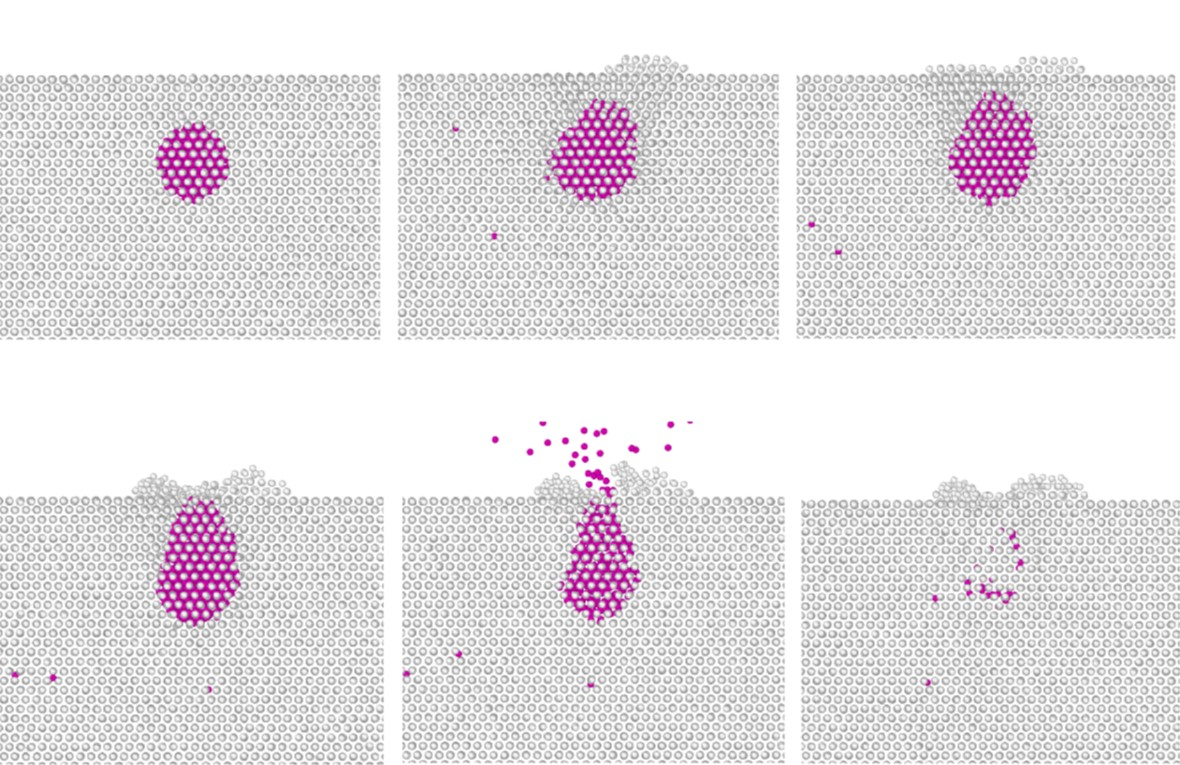
\includegraphics[width=\linewidth]{Figures/Chapter1/bubble_bursting_zhou.jpg}
    \caption{Molecular dynamics simulation of He bubble bursting in W. Reproduced from \cite{zhou_growth_2019}.}
    \labfig{bubble bursting zhou}
\end{figure}

When a bubble grows near the surface and is over-pressurised, \gls{bursting} can occur (see \reffig{bubble bursting zhou}).
As the bubble size increases via \gls{loop punching}, the W \gls{lattice} is deformed and the ligament thickness decreases.
The latter can rupture which would make all the He atoms contained in the bubble to be released to the vacuum.
This is why He \gls{bursting} is characterised by sharp drops in the He \gls{inventory} \sidecite{hammond_helium_2019}.

Sefta and co-workers observed that \gls{bursting} is more likely to happen at high temperatures.
This phenomenon contributes to surface roughening and could be the beginning of the formation of \gls{fuzz} \sidecite{sefta_helium_2013}.
Indeed, a \gls{bursting} event could either form a crater on the W surface or an empty cavity due to self-healing.
In the last case, called a \textit{pinhole} \gls{bursting} event, the cavity can be repressurised with He atoms.
Blondel et al.\ proposed to model \gls{bursting} as a stochastic function of depth in the material rather than a calculation of the bubble pressure.
They have also shown that simulation parameters have an impact on the \gls{retention} \sidecite{blondel_continuum-scale_2018}.
% These differences are mainly due to 2D effects as more bursting events occur but with smaller bubbles.
They have shown that the size of the reaction network size (using cluster dynamics) does not seem to have an influence (between 250 and 200) as the first bursting events happen with clusters of size $\text{He}_{80}$.
% Other simulation parameters (depth of the sample, pre-existing vacancies, bubble growth trajectory...) don't affect the simulations results as they converge for long time steps (100 s).

If \gls{bursting} is not included in continuum simulations, the volume fraction of He present in W could become very large and the dilute limit approximation could no longer be valid \sidecite{sefta_surface_2013}.
The correct metric for estimating \gls{bursting} probabilities must therefore be chosen with care.

\subsubsection{W tendrils or ``nano-fuzz''}

\begin{figure} [h!]
    \centering
    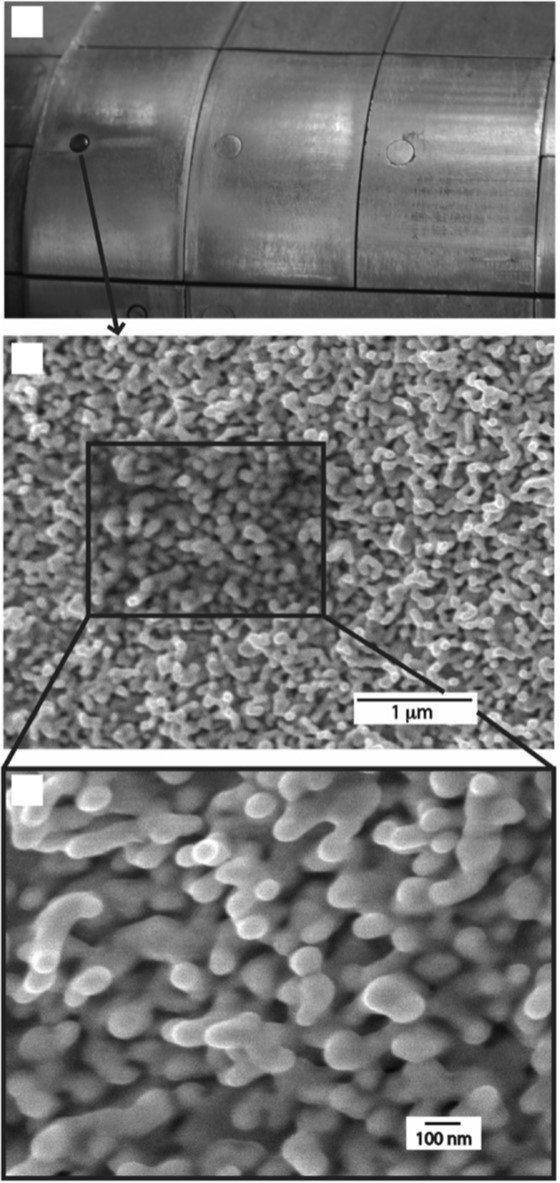
\includegraphics[width=0.5\linewidth]{Figures/Chapter1/fuzz_alcator_wright.jpg}
    \caption{W fuzz observed in Alcator C-Mod. Reproduced from \cite{wright_tungsten_2012}.}
    \labfig{w fuzz wright}
\end{figure}

In 2012, Wright et al.\ \sidecite{wright_tungsten_2012} observed the formation of nanostructures on the surfaces of the W divertor of the reactor Alcator C-mod.
These nanostructures are made of W \glspl{tendril} (see \reffig{w fuzz wright}).
These structures are called W \gls{fuzz}, nano-fuzz or even fuzzy W.
Because a small portion of the \gls{divertor} grew W \gls{fuzz}, no conclusion was made regarding its influence on the \gls{plasma} operation.
However, if these structures were to be removed during \gls{plasma} operation via erosion, W atoms could be fed into the \gls{plasma}, affecting the \gls{tokamak} performances.
Moreover, this phenomenon could increase the W dust formation in the reactor and lead to contamination and safety issues \sidecite{grisolia_tritium_2015}.

W \gls{fuzz} has been observed at high temperature (>1000K), high flux (>\SI{1e21}{He^+.m^{-2}.s^{-1}}) and long exposure (t>\SI{1e2}{s}) \sidecite{baldwin_formation_2010, nishijima_sputtering_2011}.

The reason of the \gls{fuzz} formation is still unclear but could be due to bursting events and/or accumulation of self interstitial W atoms at the surface \sidecite{baldwin_effects_2009, baldwin_helium_2008, woller_dynamic_2015, hammond_helium_2017}.
Thermal properties of the media are also impacted by the formation of W \gls{fuzz} \sidecite{wirtz_influence_2016} which could have a severe impact during ELM-like events.
After 1h of \gls{plasma} implantation, nanostructuring can be found deep in the bulk (up to several hundred of $\mu$m).
According to Baldwin and Doerner \sidecite{baldwin_formation_2010}, heavy alloying helps reduce the formation of He-induced \gls{fuzz}.

Takamura et al.\ showed \gls{fuzz} could be grown under relevant \gls{tokamak} conditions (high-flux He \gls{plasma} irradiation and surface temperature greater than \SI{1250}{K}) \sidecite{takamura_formation_2006}.
Baldwin et al.\ showed the \gls{fuzz} thickness evolved as a square root of the \gls{fluence} \cite{baldwin_effects_2009}.

\begin{figure} [h!]
    \centering
    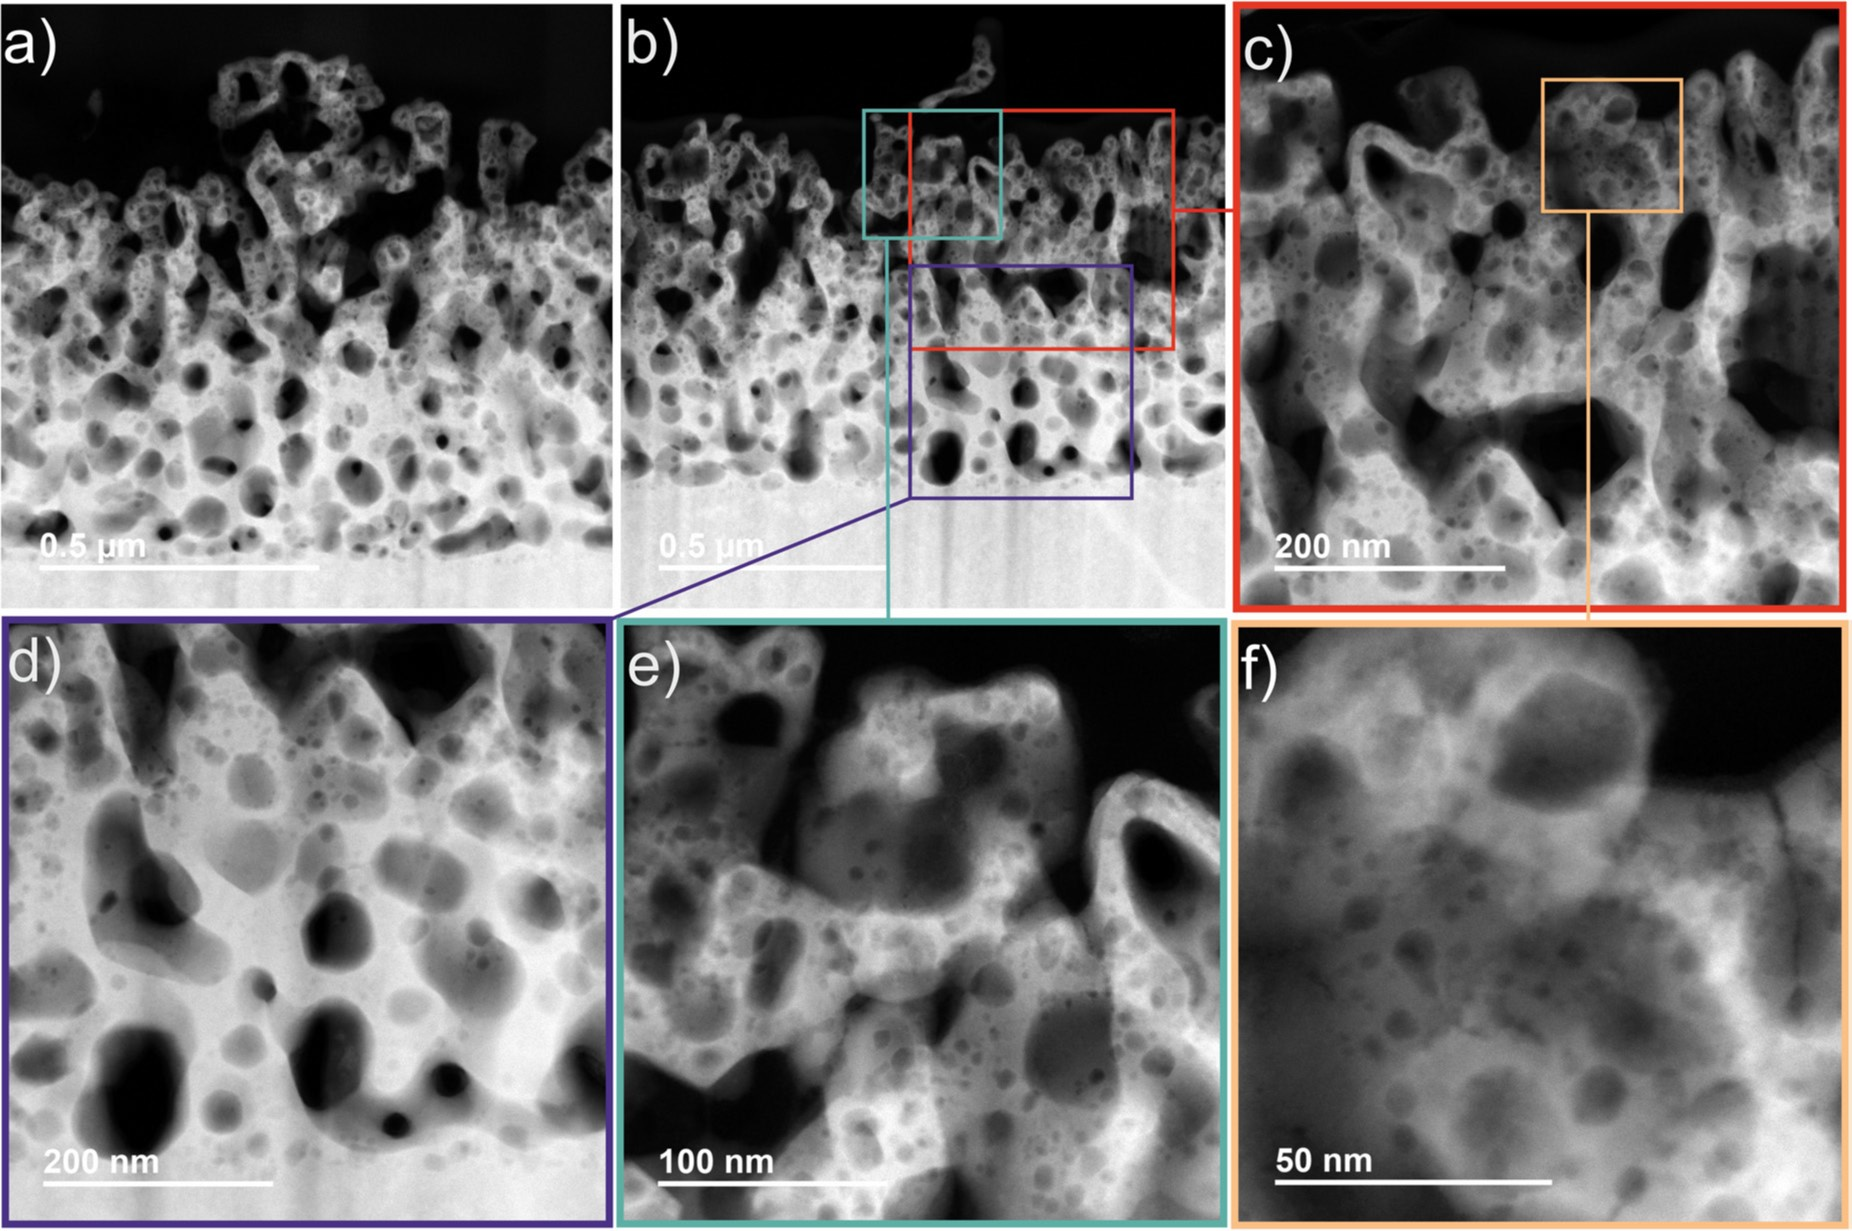
\includegraphics[width=\linewidth]{Figures/Chapter1/fuzz_mccarthy.jpg}
    \caption{Fuzzy W scanning/transmission electron microscopy images showing the presence of He bubbles in tendrils. Reproduced from \cite{mccarthy_enhanced_2020}.}
    \labfig{w fuzz mccarthy}
\end{figure}

McCarthy et al.\ studied the formation of W \gls{fuzz} (see \reffig{w fuzz mccarthy}) at helium fluences ranging from \SI{4e23}{m^{-2}} to \SI{e25}{m^{-2}}, temperatures ranging from \SI{1050}{K} to \SI{1150}{K} and He ion energies from \SI{80}{eV} to \SI{100}{eV}.
They identified different \gls{fuzz} growth regimes depending on the He \gls{fluence} due to the change in porosity of the fuzzy layer during the growth process.
The rate of growth was found to be dependent on the temperature and the state (ion or atom) of the incident He particles.

Recent modelling work also showed temperature could significantly affect the bursting of He bubbles and therefore the growth of W \gls{fuzz} \sidecite{niu_effect_2021}.

De Temmerman et al.\ concluded that temperature was the most critical parameter controlling W \gls{fuzz} growth \sidecite{de_temmerman_nanostructuring_2012}.

\subsubsection{Cracks}

The role of He implantation in cracks formation is still unclear since cracks have also been observed during pure thermal shock on W PFC \sidecite{wirtz_influence_2016}.
Under some specific conditions, cracks can close due to thermal expansion which induce frictional loads on the structure.
The formation of W nano-fuzz could also bridge those cracks as observed by Lemahieu et al.\ \sidecite{lemahieu_h/he_2016}.

\subsubsection{Reduction of thermal performances}

Several of the above phenomena can have an impact on \gls{plasma} facing materials thermal performances \sidecite{cui_thermal_2017,buzi_response_2017}.
First, having a network of bubbles will lead to a reduction of local apparent conductivity as thermal constriction will occur between the bubbles.
Therefore, for a given heat load of the surface of a PFC, temperature will likely increase.
Then, development of surface structures will be accompanied by surface roughening therefore modifying the reflectivity and emissivity \sidecite{tokunaga_synergistic_2004}.
For a given incident flux, the net radiative flux to which the surface of the component is exposed will then increase.
This could lead to reduction of the PFC heat exhaust capacity and furthermore local melting \sidecite{wirtz_influence_2016}.

% Having He transport affecting heat transfer significantly would lead to a strong coupling between the two (since He transport is strongly temperature dependent) which would imply to think of proper ways to deal with this coupling numerically.

% NOTE: an interesting study would be to investigate thermal constriction due to the presence of inhomogeneities (He bubbles) in which thermal conductivity is low compared to the one of the W.

\subsection{He/H interactions}
Lee et al.\ studied the influence of He implantation on D \gls{retention}.
They showed with Elastic Recoil Detection depth profiles (up to 40 nm) that D is trapped where He is trapped and proposed that He bubbles produce secondary defects around them which can trap D \sidecite{lee_hydrogen_2007}.
These defects can be interstitial loops produced by \gls{loop punching} or even vacancies created by stress field induced by overpressurised bubbles.
Lee et al.\ also suggested that no evidence had been found on trapping of D by chemisorption on the inner surface of a He bubble nor by molecular interaction with the He cluster.
The privileged mechanism is therefore the trapping of D in the defects made by the stress field induced by the He bubble to the crystalline structure of the W.
Bergstrom et al.\ however showed hydrogen can be located at the surface of He bubbles \sidecite{bergstrom_molecular_2017}.

It has been shown by Ueda et al.\ that He implantation (even in small amounts) greatly affects \gls{H} blistering in W \sidecite{ueda_simultaneous_2009}.
With only 0.1\% of He in the ion beam one can observe that \gls{H} blistering is completely suppressed for temperature greater than \SI{653}{K}.
At lower temperature, \gls{H} blistering occurs but is significantly reduced.
This phenomenon is due to the fact that \gls{H} migration to the bulk and accumulation at grain boundaries is avoided by He bubbles at the near surface which act as a diffusion plug for H.
The same phenomenon has been observed by Miyamoto et al.\ \sidecite{miyamoto_microscopic_2011} which contributes to reducing \gls{H} \gls{retention}.
Markelj et al.\ \sidecite{markelj_hydrogen_2017} showed however that He implantation can increase D \gls{retention} in the He clustering zone.
This suggests that observed reduction or increase of D \gls{retention} in mixed H-He \gls{plasma} experiment depend on the implantation depth.

Ialovega et al.\ performed sequential \gls{H} implantation/desorption cycles on W samples pre-damaged with He \sidecite{ialovega_hydrogen_2020}.
He bubbles were found in the near surface region (see \reffig{he bubbles ialovega}) and significantly different \gls{tds} spectra were observed after several \gls{H} implantations/desorptions (see \reffig{TDS example ialovega}).
This works gives evidence of an interaction between He and \gls{H} in \gls{W}.

\section{Problem definition}

The main focus of this PhD work is the estimation of H \glspl{isotope} \gls{retention} and permeation in \glspl{tokamak}.
We will try to answer the following questions:
\begin{itemize}
    \item How does the tritium \gls{inventory} evolve over the lifespan of the fusion reactor?
    \item Does it remain within the safety limits?
    \item What is the impact of the presence of helium?
\end{itemize}

Due to the time scales at play and the complexity of the components, answering these questions experimentally is complex.
Numerical models can however be used to simulate components over long time scales and with complex geometries.
However, the tools currently available did not meet the requirements of either dimensionality, physics, performance or availability.

Numerous simulation tools have been developed throughout the years (see \reftab{code comparison}).
Most of these codes are not able to run multimaterial and/or multidimensional simulations.
These features are however essential to fully simulate monoblocks (see \refsec{divertor section}).
Many of them rely on the \gls{fdm} whereas \acrshort{hit} \sidecite{candido_integrated_2020}, Abaqus \sidecite{benannoune_multidimensional_2020} and \gls{achlys} \sidecite{dixon_aurora-multiphysicsachlys_2021} rely on the \gls{fem}.
Moreover, some do not have an integrated heat transfer solver - essential for an accurate estimation of temperature fields and therefore thermally activated processes.
Some of these codes rely on proprietary software like Abaqus or COMSOL for \acrshort{hit} - limiting their accessibility and scalability (parallel computing).
The code \gls{achlys} meets all these requirements and is the only one available open-source but was only released in mid 2021.
Finally, good computing performances were required in order to simulate the full \gls{divertor}.
This ruled out the use of Abaqus in its current state as it was initially designed for thermo-mechanical simulations.

For all these reasons, the \acrshort{festim} code was developed and used to conduct this PhD research.

\begin{table*} [h]
    \centering
    \begin{tabular}{L{2cm} L{0.5cm} L{0.5cm} L{0.6cm} L{1.7cm} l l l }
        & 1D & 2D & 3D & Multimaterial & Heat transfer & Open-source & Programming language \\
        \hline \\
        \acrshort{tmap7} \cite{longhurst_tmap7_2008} & $\checkmark$ & & & $\checkmark$ & & & Fortran\\
        \\
        \acrshort{hiipc} \cite{sang_modelling_2012} & $\checkmark$ & & & & $\checkmark$ & & Fortran\\
        \\
        \acrshort{crds} \cite{matveev_reaction-diffusion_2018} & $\checkmark$ & & & & & & Mathematica \\
        \\
        \acrshort{mhims} \cite{hodille_study_2016} & $\checkmark$ & & & & & & Fortran \\
        \\
        \acrshort{tessim} \cite{schmid_transport_2014} & $\checkmark$ & & & $\checkmark$ & & & \\
        \\
        \acrshort{hit} \cite{candido_integrated_2020} & $\checkmark$ & $\checkmark$ & $\checkmark$ & $\checkmark$ & $\checkmark$ & & COMSOL interface\\
        \\
        Abaqus \cite{benannoune_multidimensional_2020} & $\checkmark$ & $\checkmark$ & $\checkmark$ & $\checkmark$ & $\checkmark$ & & Fortran user subroutines\\
        \\
        \gls{achlys} \cite{dixon_aurora-multiphysicsachlys_2021} & $\checkmark$ & $\checkmark$ & $\checkmark$ & $\checkmark$ & $\checkmark$ & $\checkmark$ & C++\\
        \\
    \end{tabular}
    \caption{Comparison of some hydrogen transport modelling tools.}
    \labtab{code comparison}
\end{table*}

\begin{itemize}
    \item \textbf{\refch{Chapter2}} \newline
The first part of this work was to develop a model and a simulation tool - \acrshort{festim} - capable of solving hydrogen transport problem in 2D/3D.
This Chapter will describe the mathematical models used in \acrshort{festim} as well as the global numerical implementation.
Finally, it will detail the analytical verification and experimental validation strategy.
This last point includes a code comparison with the reference code \acrshort{tmap7}.
    \item \textbf{\refch{Chapter3}} \newline
This Chapter will focus on estimating the tritium \gls{retention} in \glspl{monoblock}.
To this end, a \acrshort{festim} model of \acrshort{iter}-like \gls{monoblock} will be developed.
A behaviour law linking the \gls{monoblock} \gls{inventory} to exposure conditions (surface concentration and surface temperature) will be obtained.
    \item \textbf{\refch{Chapter4}} \newline
The next stage is to scale up from a \gls{monoblock} model to a full \gls{divertor} model.
The behaviour law obtained in \refch{Chapter3} will be coupled to \gls{plasma} simulations (providing distributions of exposure conditions).
The \gls{inventory} of the \acrshort{iter} and WEST \glspl{divertor} will be computed for several \gls{plasma} scenarios.
    \item \textbf{\refch{Chapter5}} \newline
Finally, the influence of helium exposure and the presence of helium bubbles was studied.
To this end, a finite element solver was first developed to simulate helium transport and clustering in tungsten.
This code was compared to the Xolotl code \sidecite{blondel_continuum-scale_2018}.
This helium transport code was then coupled to \acrshort{festim} to estimate the potential impact of helium on the tritium \gls{inventory} estimations.
\end{itemize}
